\documentclass[12pt]{report}
\usepackage{graphicx}
\usepackage{subfigure}
\usepackage{url}
\usepackage{color}
\usepackage{fullpage}
%\usepackage{geometry} % see geometry.pdf on how to lay out the page. There's lots.
%\geometry{letterpaper} % or letter or a5paper or ... etc
% \geometry{landscape} % rotated page geometry

% See the ``Article customise'' template for come common customisations

\title{HPS SVT Operations Manual \\ v1.0}
\author{SVT On-Call Cell Phone: 757-541-7539 \\ 
Authors: \\
Per Hansson, John Jaros, Takashi Maruyama, Omar Moreno,\\ Tim Nelson\footnote{contact person for this document}, Marco Oriunno, Sho Uemura}
\date{March 8, 2015} % delete this line to display the current date

%%% BEGIN DOCUMENT
\begin{document}

\maketitle

\section{Contact List}

\begin{center}
\begin{tabular}{lc}
\hline \hline 
System & Experts \\
\hline
General expert & Tim Nelson \\
SVT DAQ & Pelle Hansson \\
SVT EPICS controls & Pelle Hansson, Wesley Moore \\
MPOD power supply & Sho Uemura \\
PLC interlocks & Brian Eng \\
Cooling & Sho Uemura \\
 \hline \hline
\end{tabular}
\end{center}

\chapter{System Description}

The SVT, shown in Figure~\ref{fig:SVT}, uses 6 layers of silicon extending from 10 cm to 90 cm downstream of the target inside of the PS vacuum chamber to measure charged particle trajectories.  
%=======================
\begin{figure}[htbp]
\begin{center}
    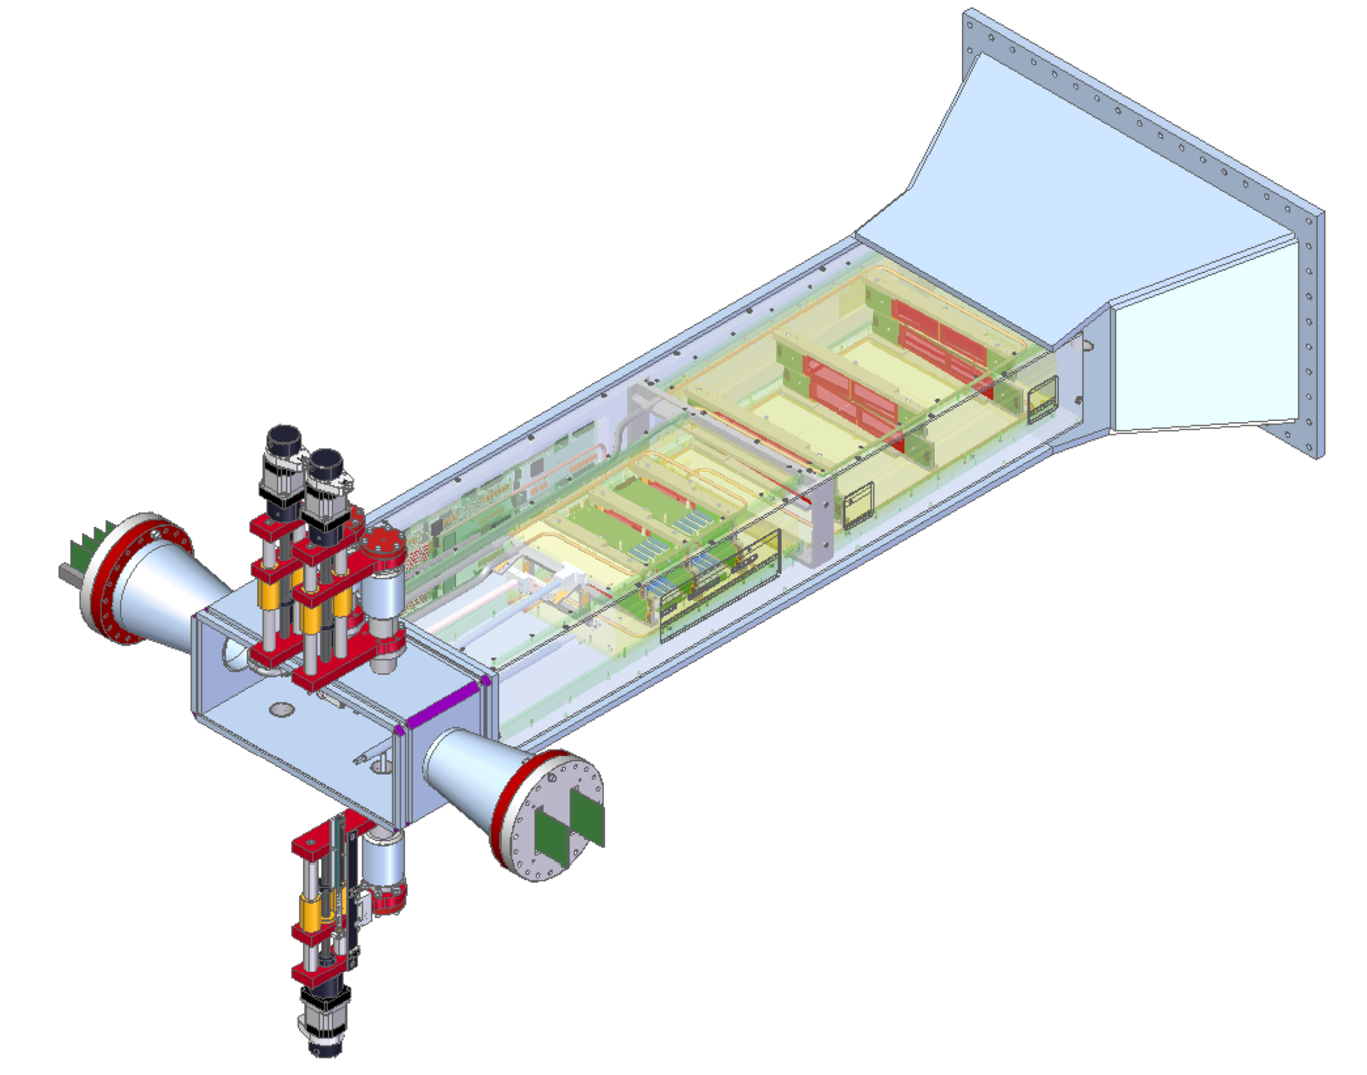
\includegraphics[width=7cm]{SVT}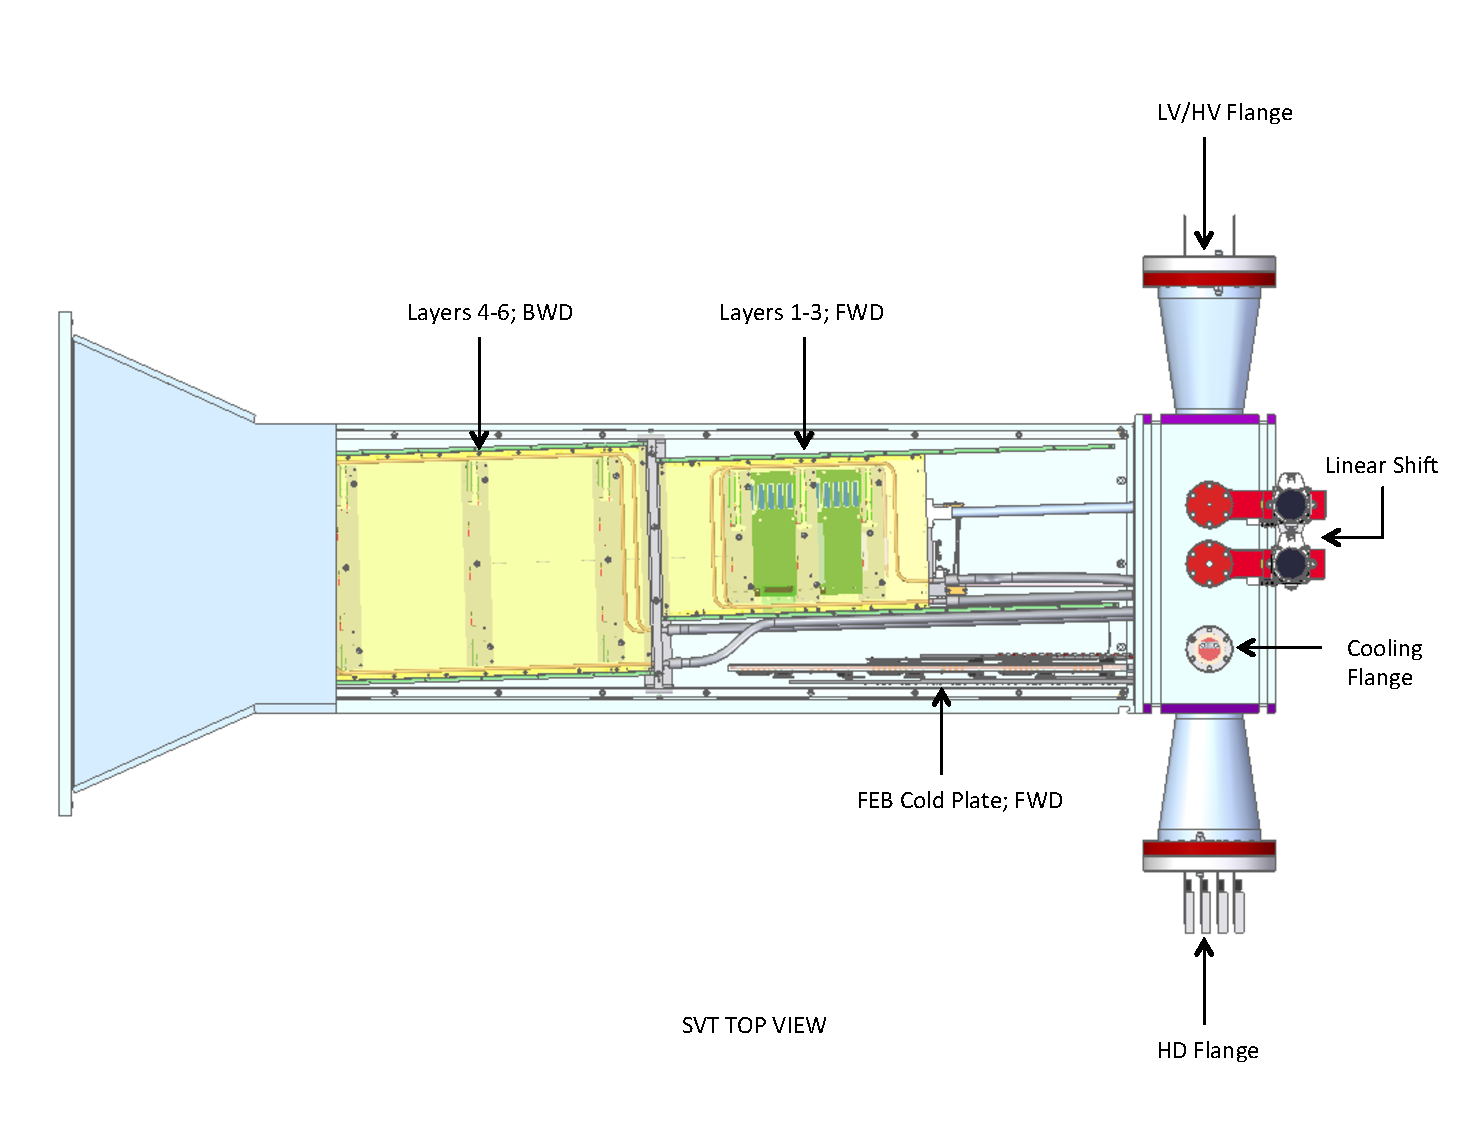
\includegraphics[width=7cm]{SVT_top}
\caption{The SVT shown inside of the pair spectrometer vacuum chamber.  The beam enters through the flange in the front of the vacuum box extension that houses services for the SVT. }
\label{fig:SVT}
\end{center}
\vspace*{-5mm}
\end{figure}
%=======================
To accommodate the passage of the beam, the SVT is built in two halves, top and bottom, so that each layer consists of a pair of modules, one above and one below the beam plane.  Each module uses silicon microstrip sensors placed back-to-back with a small stereo angle between sides to provide 3-d space points for the hits in a module.  Modules for layer 1-3 have a single sensor on each side with readout at one end, while those for layers 4-6 are longer, with a pair of sensors on each side and readout at both ends.

Modules are supported in groups of three by a set of four support plates, as shown in Figure~\ref{fig:L1-3_bottom}. The top and bottom support plates for the back half of the SVT (layers 4-6) are stationary.  However, the supports for layers 1-3 can be opened and closed vertically around the beam, rotating around hinges behind layer 3 and moved by levers extending upstream to a pair of linear shifts outside of the magnet. The support plates are kinematically mounted inside a support box that installs into the pair spectrometer (PS) vacuum chamber, shown in Figure~\ref{fig:SVT_Box}.
%=======================
\begin{figure}[htpb]
\subfigure[\label{fig:L1-3_bottom}The lower support plate for Layers 1-3, showing the silicon (red) and readout electronics (green) of the modules, as well as the motion lever for opening and closing the SVT and the SVT beam scan wires.]
{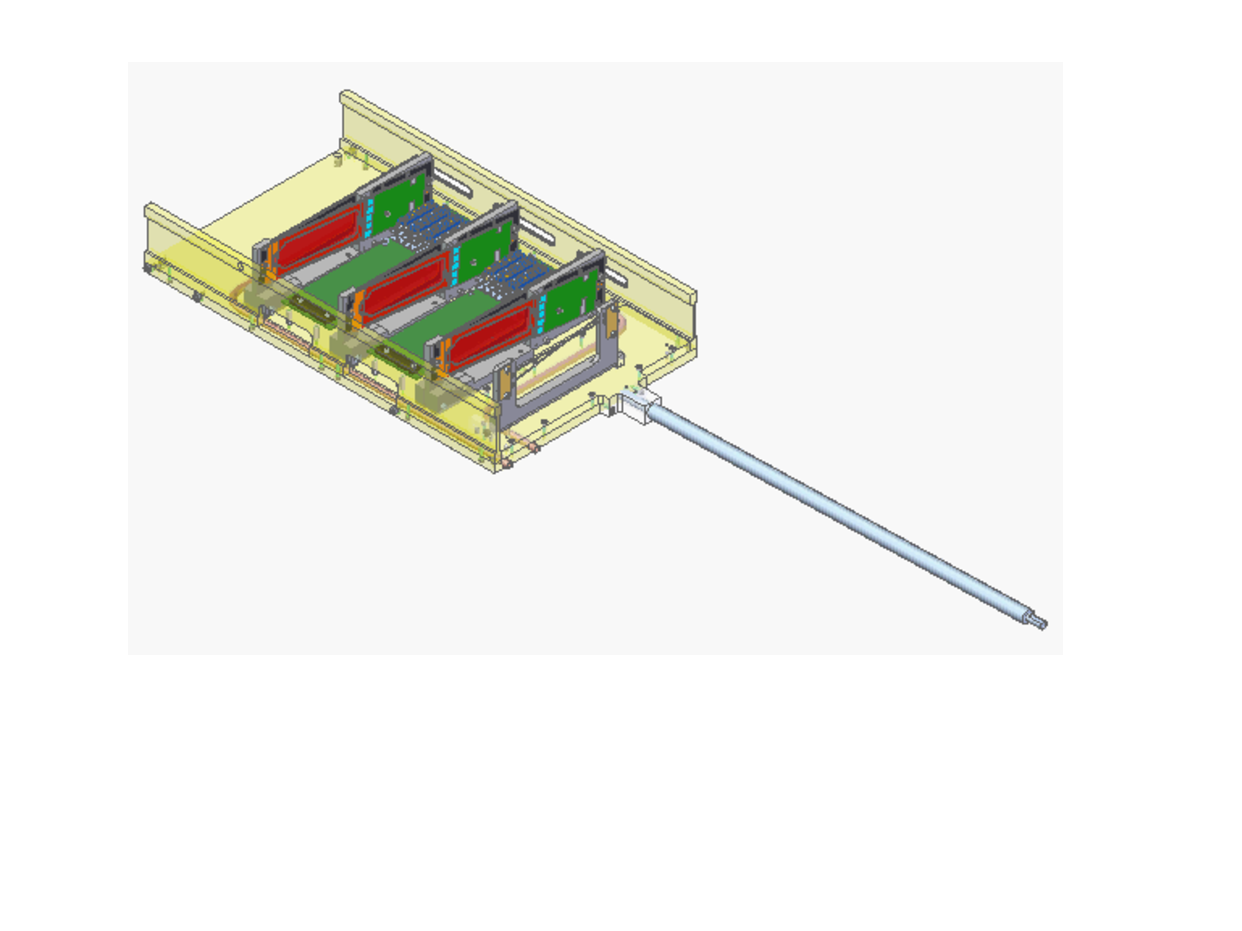
\includegraphics[width=6.5cm]{L1-3_bottom}}
\hspace{0.5cm}
\subfigure[\label{fig:SVT_Box}The SVT support box which contains the upper and lower support plates for Layers 1-3 and Layers 4-6, as well as the cooling plate housing the Front End Boards of the SVT DAQ.]
{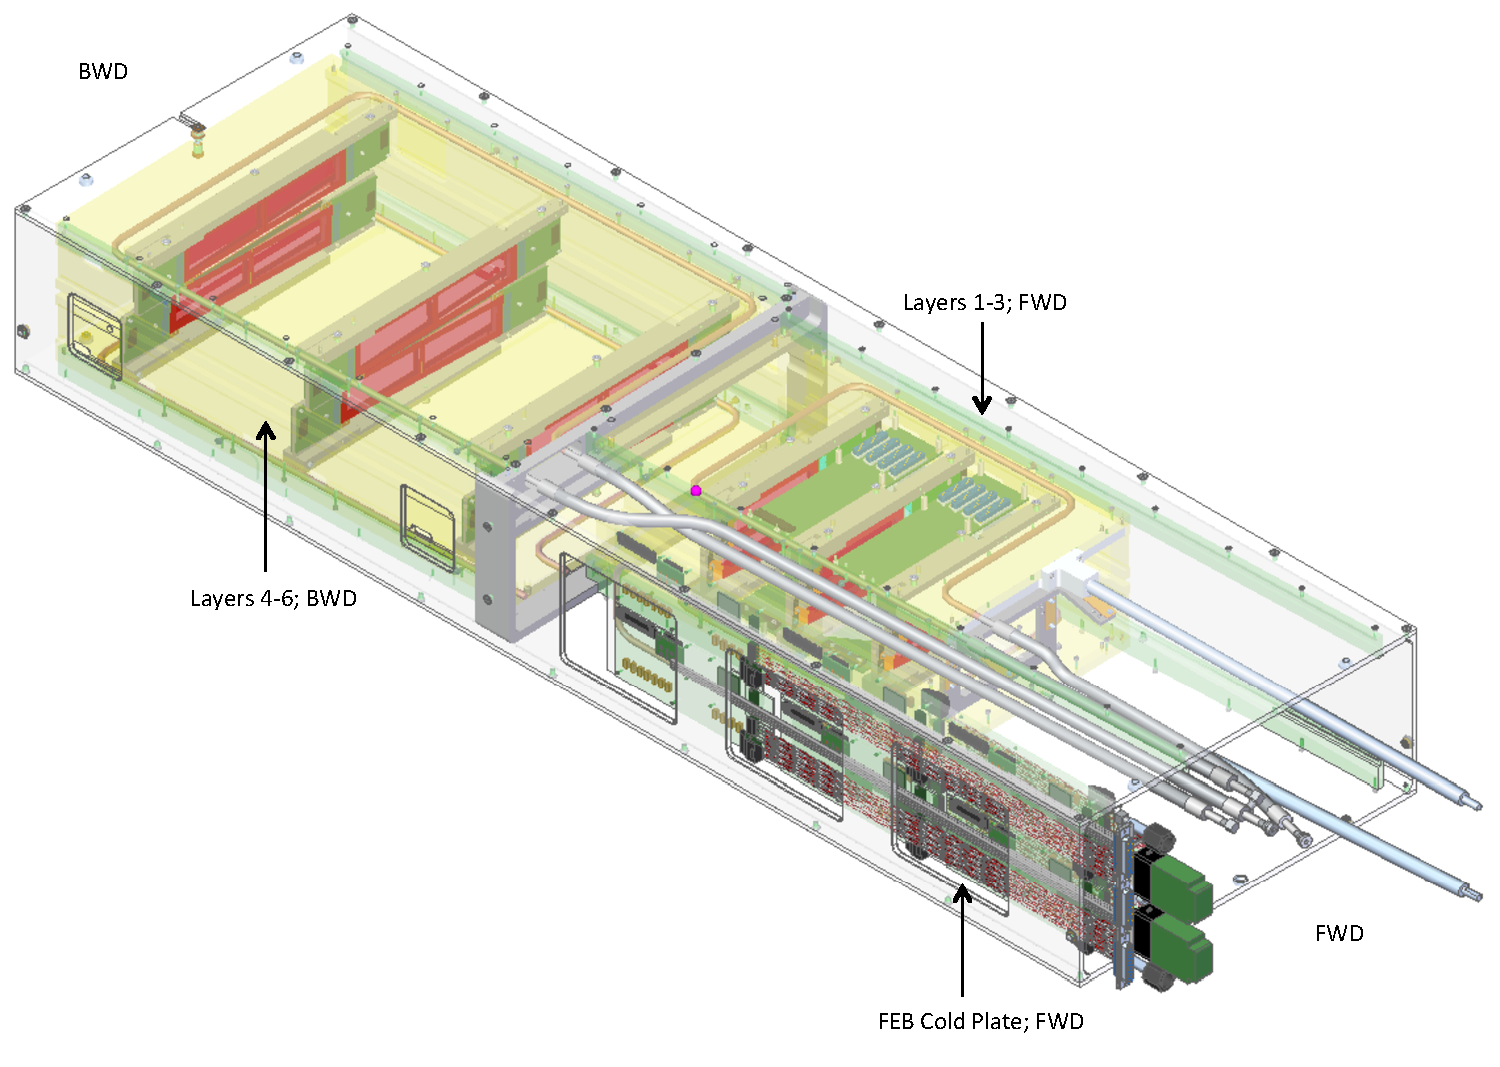
\includegraphics[width=6.5cm]{SVT_Box}}
\caption{Key sub-assemblies of the SVT.}
\end{figure}
%=======================

The first stage of readout electronics is located on a hybrid circuit board at the end of each sensor.  Multiplexed analog signals from these boards are digitized by a set of 10 Front End Boards (FEBs) mounted to a separate cooling plate inside the SVT support box. Each FEB can control 4 hybrid/sensor units: a single module in layers 4-6 and either one or two modules in layers 1-3. The FEBs also control the hybrids, provide regulated low-voltage power from a single input, and pass externally generated bias voltages (HV) through to the sensors.   The FEBs communicate with a set of 4 Signal Flange Boards (SFB), up to three per SFB, which transmit digital signals through the vacuum penetration.  The exterior side of each flange board converts digital to optical signals for communication with the RCE DAQ.  Power to the FEB are routed through a pair of Power Flange Boards, one for LV and one for HV, supplied by a Wiener Mpod power supply modules in a crate on the pie-tower.

Cooling for the SVT is provided by a pair of chillers; one for the hybrids and sensors that operates at -10 $^\circ$C and one for the FEBs that operates at room temperature.  The FEBs have a single cooling loop, while the hybrids and sensors have two loops, one for the top and one for the bottom half of the SVT, where each of these loops runs first through the support structure for layers 1-3 and then through the structure for layers 4-6.  There are temperature sensors on every hybrid as well as sensors in the FEBs. The linear shifts, the cooling penetrations, and the signal/power penetrations are all located on a set of flanges on an extension vacuum box mounted to the upstream end of the PS vacuum chamber and which connects to the upstream beam line.

Since the SVT sensors are close to the beam, some attention to beam conditions is required prior to turning the SVT on and taking data. A number of systems provide the information used to assess whether beam conditions allow SVT operation. These systems include beam position monitors along the beamline, wire scanners located upstream of the HPS chicane, the wire attached to the SVT itself, a protection collimator located just upstream of the HPS chicane, and beam halo counters located along the beamline downstream of the collimator and signals from the HPS ECal which serve together as beam background monitors.  A detailed description of these systems and their operation can be found in the Beamline Operations Manual.






\section{Voltages}
The power and bias needed to operate the SVT is supplied by low voltage and high voltage power supply modules inside a 10-slot Wiener MPOD crate, see Fig.~\ref{fig:ec_crate}. 
\begin{figure}
\begin{center}
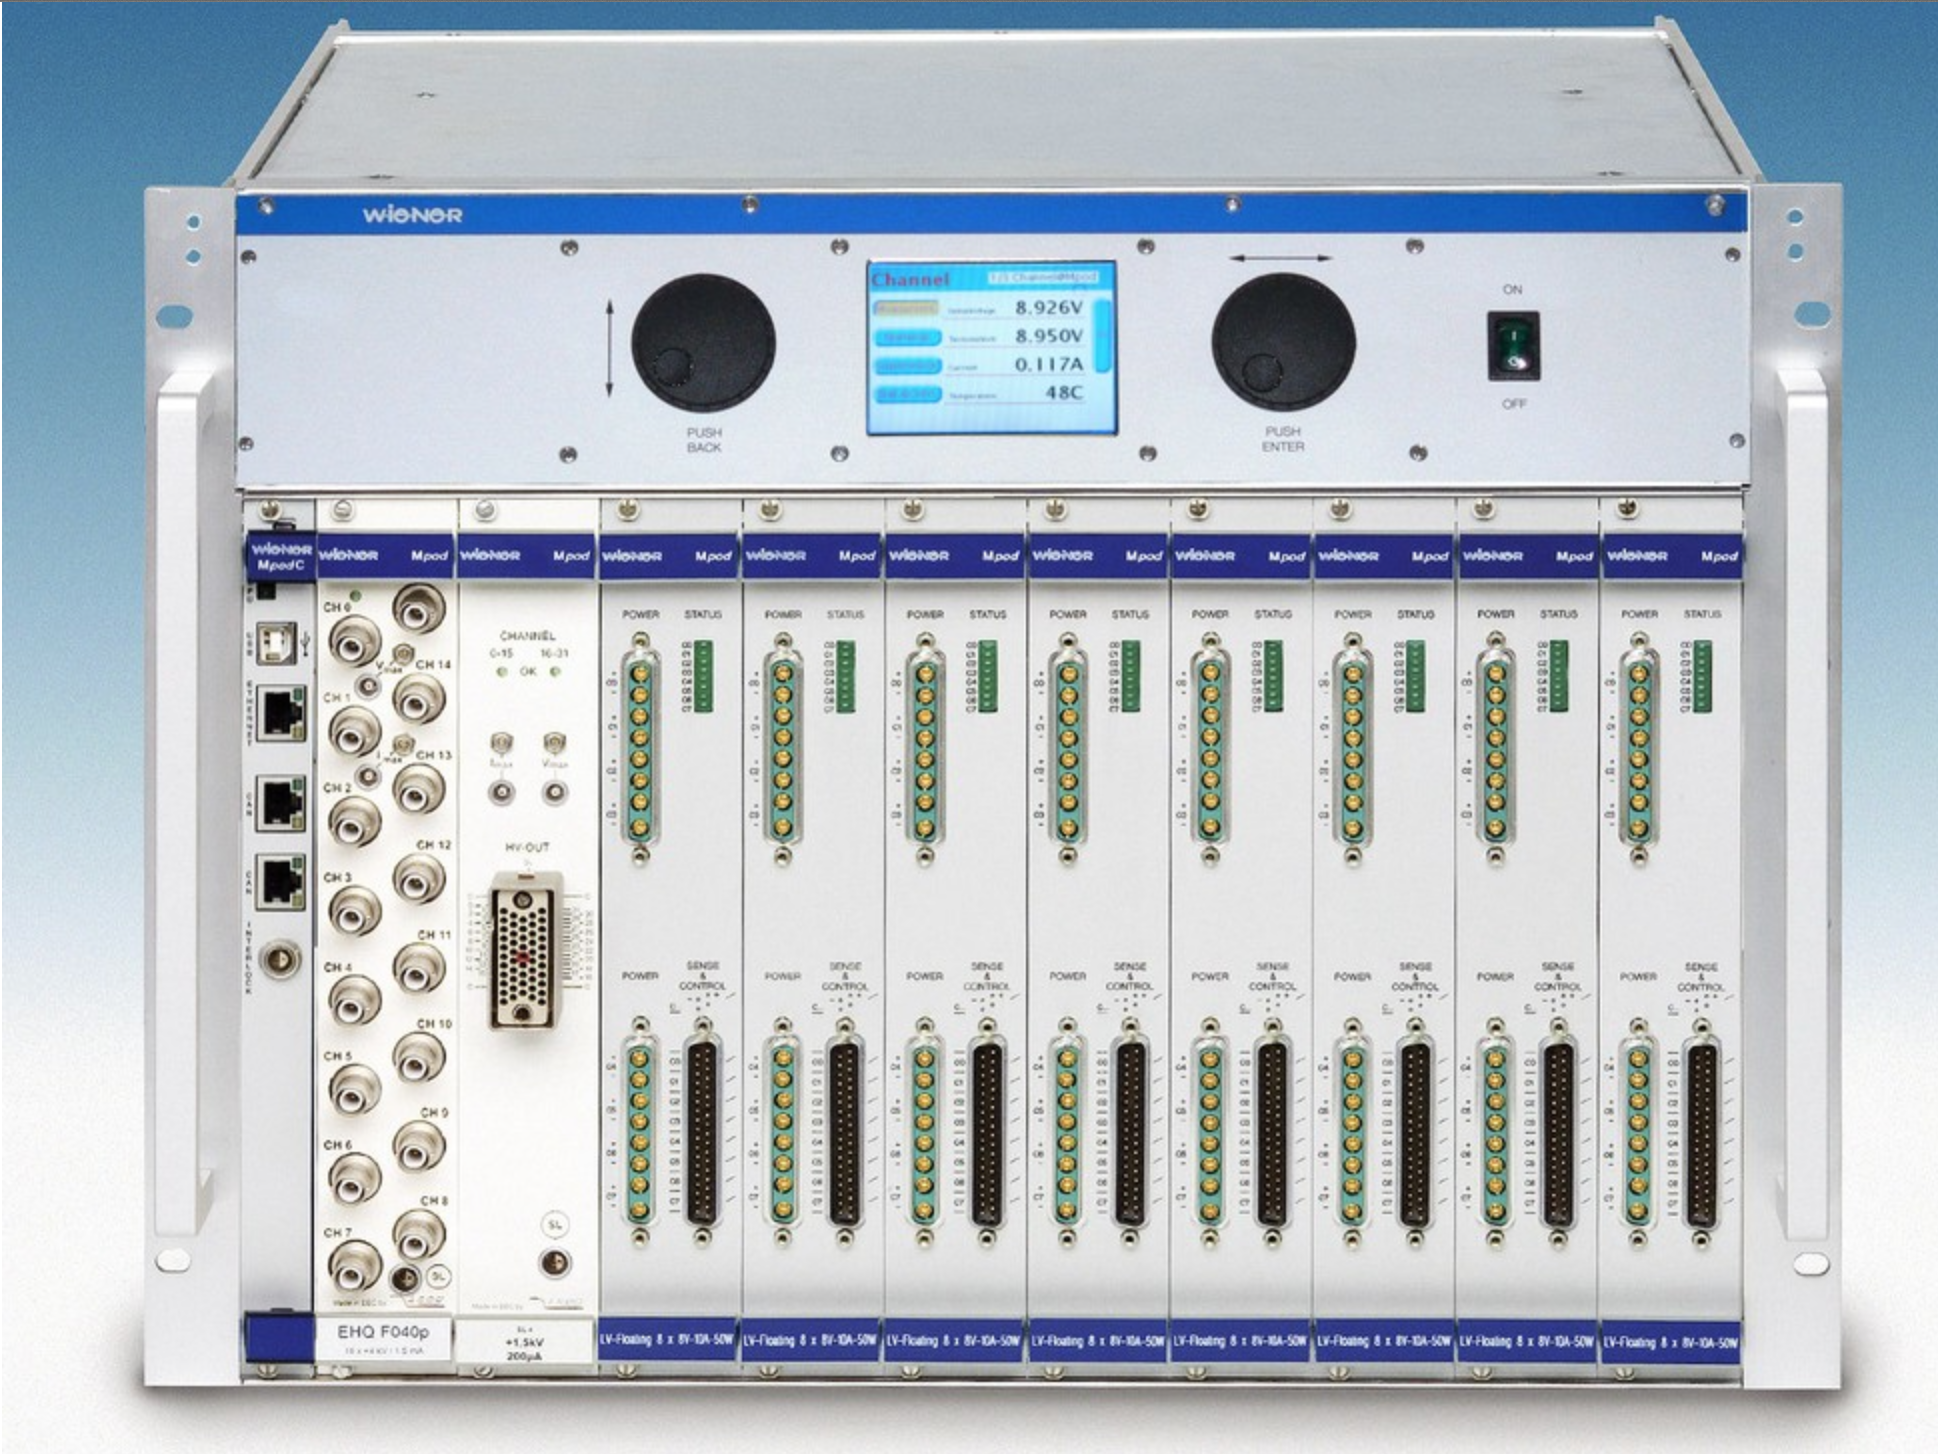
\includegraphics[width=10cm]{ec_create.png}
\caption{\label{fig:ec_crate}The Wiener power supply crate for the SVT.}
\end{center}
\end{figure}
The crate is located in a rack in the pie tower with PTFE (teflon) insulated twisted pair copper wires used to bring power to the SVT in the Hall-B alcove. 

The low voltage power is supplied by Wiener MPV8008I low voltage power supply modules. Each module has 8 output channels (floating, with sense lines).
Each of the five modules supplies power to two FEBs. 

ISEG EHS F201p\_805F high precision high voltage modules provide the reverse bias voltage to the silicon sensors of the SVT. Each module has 16 output channels (floating). The three modules each supply bias to 12 sensors: SVT L1-3, L4-6 top or L4-6 bottom.  

The last two slots in the crate are occupied by spare modules (one LV and one HV).

\subsection{Control and Monitoring}
The SVT power supply and bias is fully controlled through GUIs to the EPICS control system. 
EPICS controls the MPOD crate directly through its SNMP interface which supply the FEBs with power. 
The FEBs regulate and distribute power down to the hybrid boards of the SVT sensor modules. 
The control and monitoring of the hybrid power (and temperature) is handled by an EPICS IOC running on the SVT DAQ crate. 

%It is important to note that having cooling running is a prerequisite for any power being supplied to the SVT and configuration of the FEB are prerequisite for powering any hybrids.
Both cooling systems must be running before the MPOD can be turned on; this is enforced by an interlock. 
Also, the FEBs must be configured before any hybrids can be powered.

\section{Cooling and Interlocks}
The SVT cooling system, summarized in Table~\ref{tab:cooling} and Figure~\ref{fig:cooling_diagram}, controls the temperature of the sensors and removes heat dissipated by the electronics. 
%===================
\begin{table}[ht]
\begin{center}
\begin{tabular}{lccc}   
\hline \hline 
Location & Set Point & Resistive Load & Radiative Load \\      
\hline
SVT modules & -10 $^\circ$C & 75 W & 10 W  \\
Piping to SVT modules & -20 $^\circ$C & 100 W & 0 \\
Set point, SVT chiller & -20 $^\circ$C & - & - \\
Front End Boards & 25 $^\circ$C & 100 W & 0  \\
Set point, FEB chiller & 20 $^\circ$C & - & - \\
 \hline \hline
\end{tabular}
\caption[]{SVT cooling design parameters.}
\label{tab:cooling} 
\end{center}
\end{table}
%===================
%=======================
\begin{figure}[htbp]
\begin{center}
    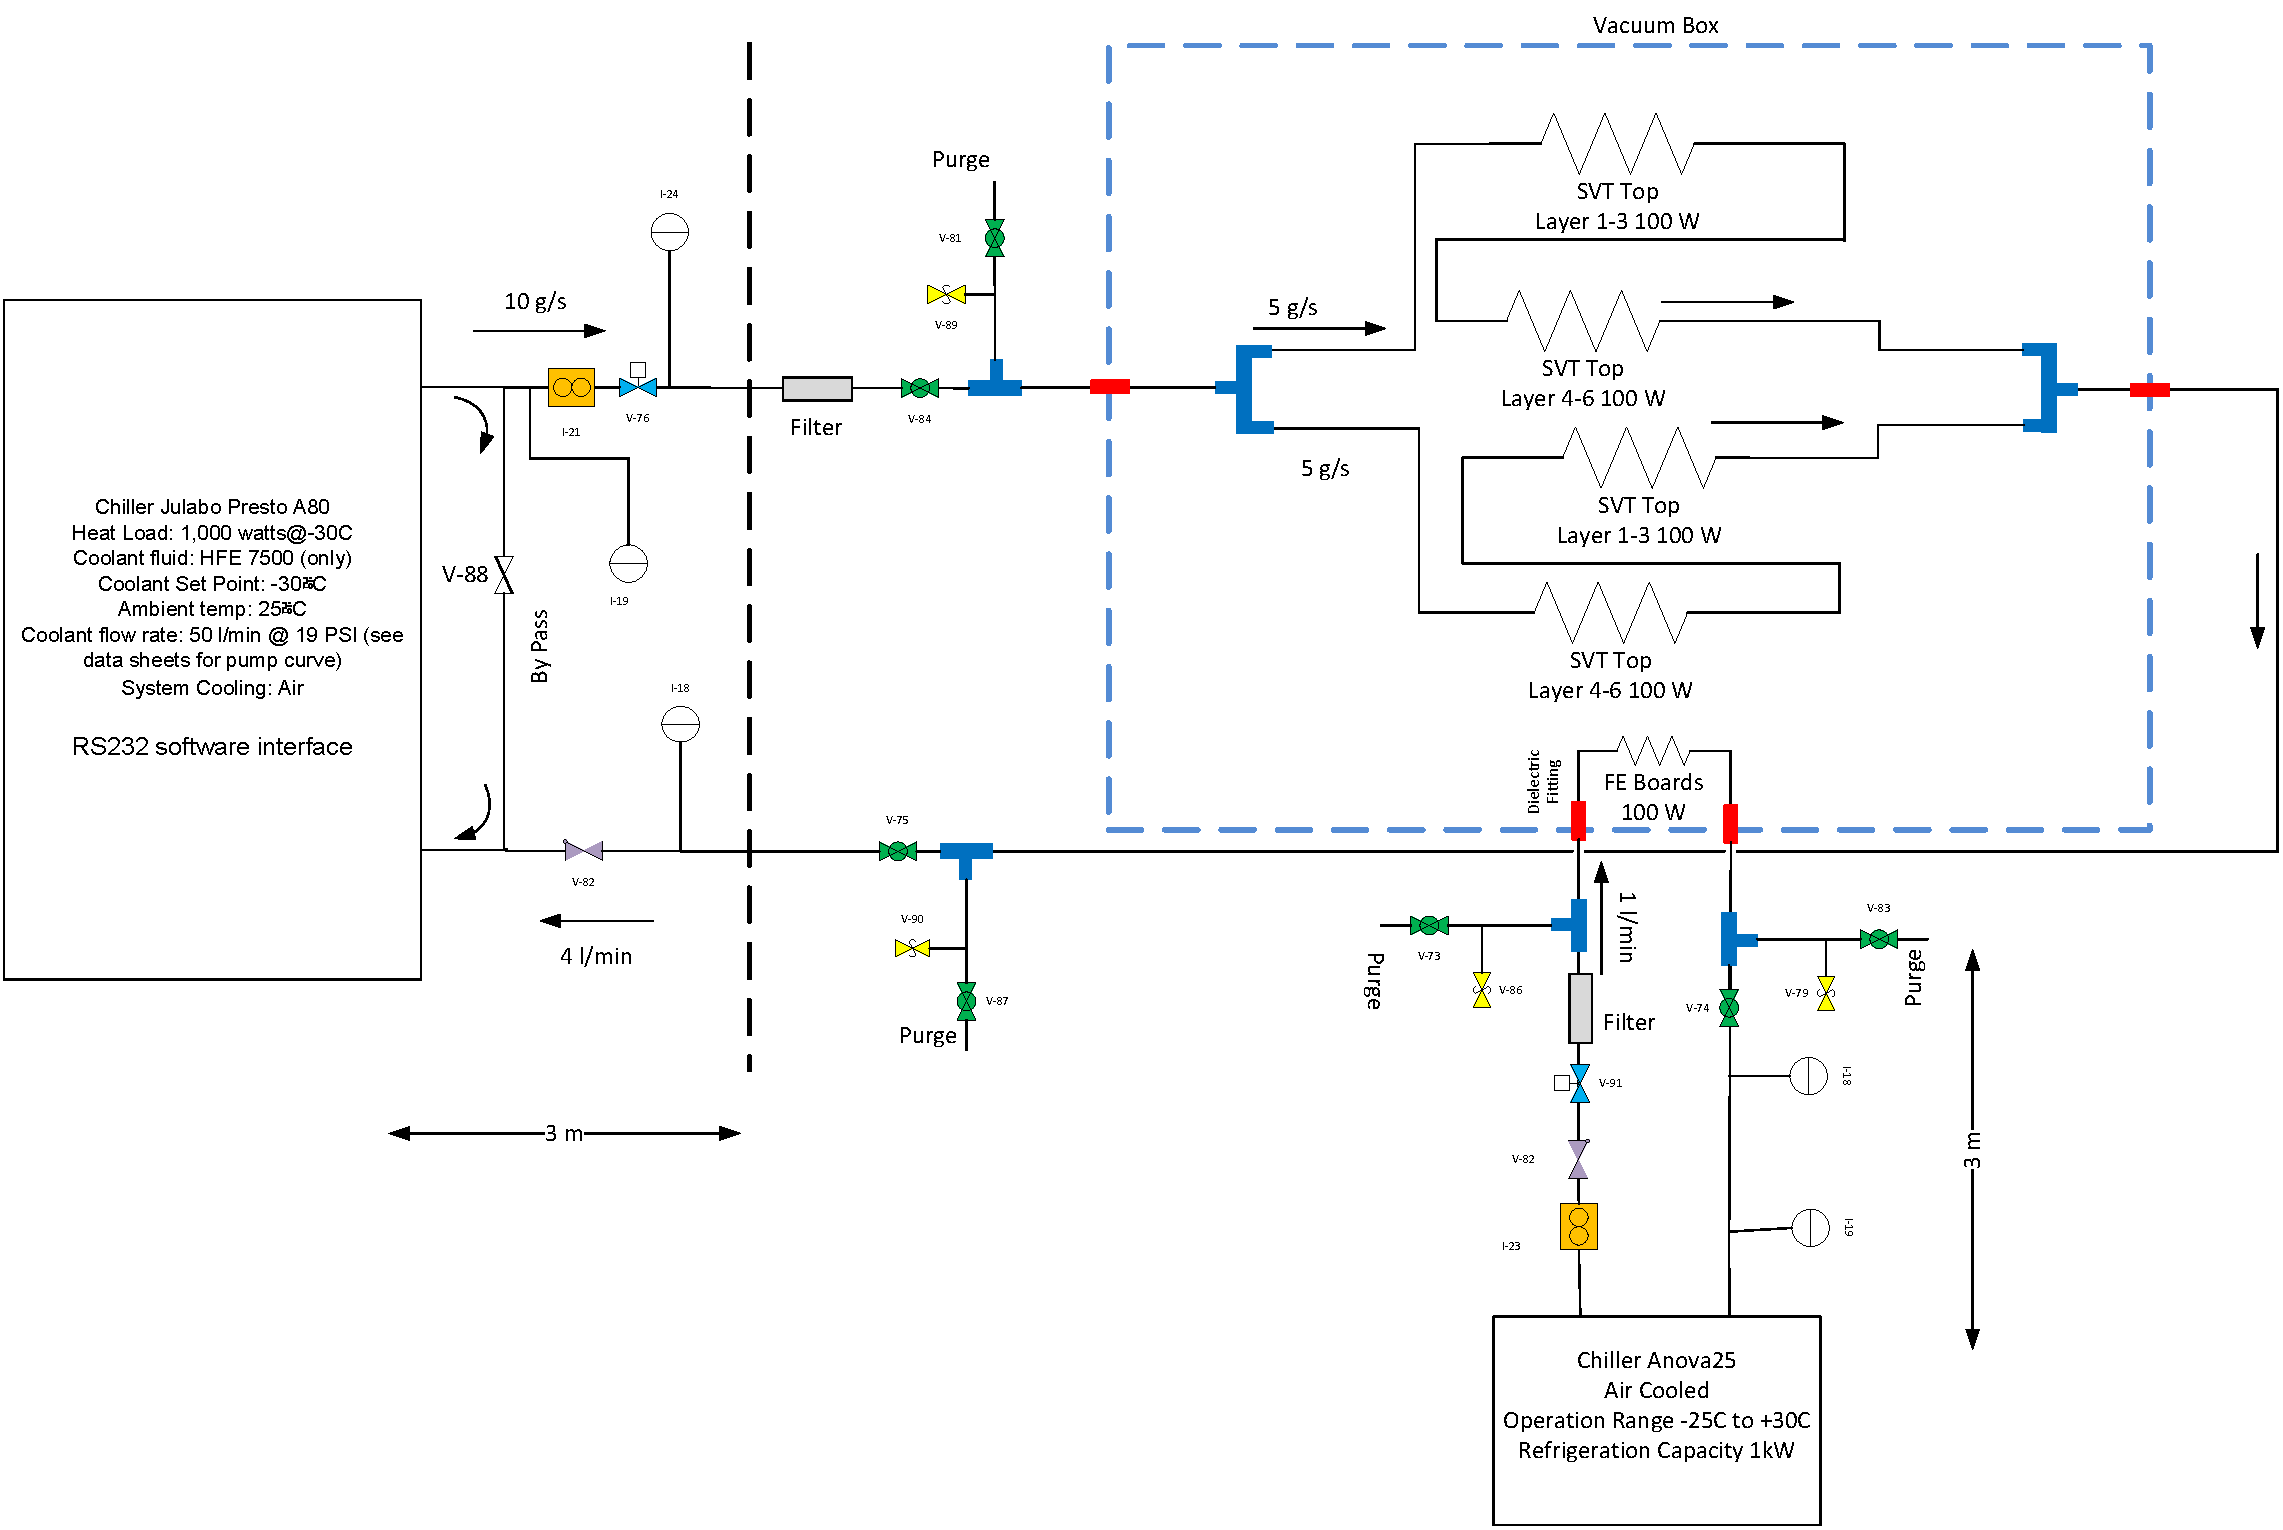
\includegraphics[width=\textwidth]{cooling_diagram}
\caption{The SVT cooling system.}
\label{fig:cooling_diagram}
\end{center}
\end{figure}
%=======================
Since the SVT is in vacuum, the cooling system is key for the safety and performance of the detector. The main heat sources are the sensor modules and their hybrid circuit boards and the Front End Boards (FEBs) which distribute power and DAQ to reduce the number of wires that must penetrate the vacuum flanges. An additional heat load results from the radiative heat exchange between the SVT U-support and the detector vacuum. The sensor modules need to be controlled to a sub-zero temperature, while the FEBs needs to be only thermally managed, removing the heat dissipated and keeping the active components to safe temperature, slightly above room temperature. For this reason it has been decided to have two separate chillers with independent loops and controls. The dew point in Hall B is expected to be at ~18 $^\circ$C. The cold line from the sensor chiller to the vacuum box will be insulated with 1� thick, non-flammable Armaflex.

The cooling loop for the sensor modules is connected to a Julabo Chiller, Model Presto A80, which will be set at -30 $^\circ$C. The heat transfer fluid is HFE-7000, a Fluorinert engineered fluid long used as heat transfer media for cooling applications. A bypass valve is placed at the chiller to manually adjust the mass flow. The inlet and the outlet lines pass through flanges on the detector vacuum box, where they are split after the feed trough to provide cooling in series to the top and the bottom parts of the detector. The cooling pipes in vacuum are flexible metal hoses from the vacuum feed through to the detector, while the cooling lines built in the detector are 0.25" rigid copper pipe. The flexible lines are brazed on one end to the rigid copper pipes of the detectors and connected with Swagelok fittings to the vacuum feedthroughs on the other end. The cooling feed through have a ceramic transition spool to insulate electrically the cooling line from the vacuum box. Dielectric fittings to break the electrical continuity of the cooling loop are placed outside the vacuum.  The drain ports are placed in proximity of the cooling feedthroughs together with two release valves, on the main supply and the main return line.
In addition to the filter of the chiller, a second filter is located on the main supply line. A check valve is at the end of the main return line, just before the bypass. The estimated operating mass flow of the system without bypass is ~ 10 g/s, providing 5 g/s per cooling channel with a pressure drop ~1 bar.  The cooling loop inside vacuum is pneumatically tested up to 20 bars without showing any sign of failure.

All the instrumentation to control the cooling system will be placed in air, close to the chillers, with an identical layout for the two, as shown in Figures~\ref{fig:cooling_diagram}. 


One mechanical pressure dial gauge is located after the bypass, on the main supply line. Two Pt100 temperature sensors are located at the inlet and the outlet of the chiller. A paddlewheel flow meter located after the bypass provide the value of the flow going to the detector. A solenoid valve after the flow meter is stopping the cooling flow when requested by the slow control system, like in case of leaks. The temperature sensors and the flow meter are interfaced with the Slow Control as diagnostic, while the solenoid valve is interlocked. Additional diagnostic is available through the temperature sensors built-in the SVT modules and the functional parameters of the chillers like set point pump pressure, mass flow which are controlled through an RS232 software interface.



\subsection{Sensors and inputs}
\subsubsection*{FEB cooling loop}
\begin{itemize}
    \item To PLC: Flow switch (adjustable setpoint, set around 10 GPH with reference to flow meter) at chiller return
    \item To PLC: 2x RTD on supply and return, near vacuum feedthroughs
    \item Through SVT DAQ: temperature sensors on FEBs
    \item From FEB chiller (via RS-232): temperature readout, status
    \item Local readout only: flow meter, next to flow switch
\end{itemize}
\subsubsection*{SVT cooling loop}
\begin{itemize}
    \item To PLC: Flow switch (fixed setpoint, 0.25 GPM) at chiller return
    \item To PLC: 2x RTD on supply and return, at manifold (before lines split to top and bottom halves of the SVT)
    \item Through SVT DAQ: temperature sensors on hybrids
    \item From SVT chiller (via RS-232): temperature readout, outlet pressure, status
    \item Local readout only: 2x pressure gauges, on supply and return at manifold
\end{itemize}

The sensors with PLC or RS-232 readout are monitored through the EPICS slow controls system and displayed in the monitoring GUIs for the chillers and the PLC.
The SVT alarm handler has alarms defined for the temperatures: see the SVT monitoring section.

\subsection{Control outputs}
The PLC and chillers can be controlled through EPICS. These control outputs can be used in PLC or EPICS interlocks.
\subsubsection*{FEB cooling loop}
\begin{itemize}
    \item From PLC: Solenoid valve at chiller outlet
    \item On FEB chiller (via RS-232): start/stop, temperature setpoint, pump speed
\end{itemize}
\subsubsection*{SVT cooling loop}
\begin{itemize}
    \item From PLC: Actuated ball valve at chiller outlet
    \item From PLC: Chiller circuit breaker
    \item On SVT chiller (via RS-232): start/stop, temperature setpoint, pump power
\end{itemize}
\subsubsection*{Voltages}
\begin{itemize}
    \item From PLC: MPOD enable signal (shuts down all LV and HV channels)
    \item From MPOD IOC: Controls for individual MPOD channels
\end{itemize}



\subsection{Interlocks}
\label{sec:svt_power_monitoring_alarm_interlocks}

To safely operate the SVT, the power supplies are included in an interlock system that triggers a fast shutdown of the power supply crate based on a set of conditions. A schematic view of the interlock system that triggers a SVT power supply interlock signal is shown in Fig.~\ref{fig:svt_interlock_diagram}. 
\begin{figure}
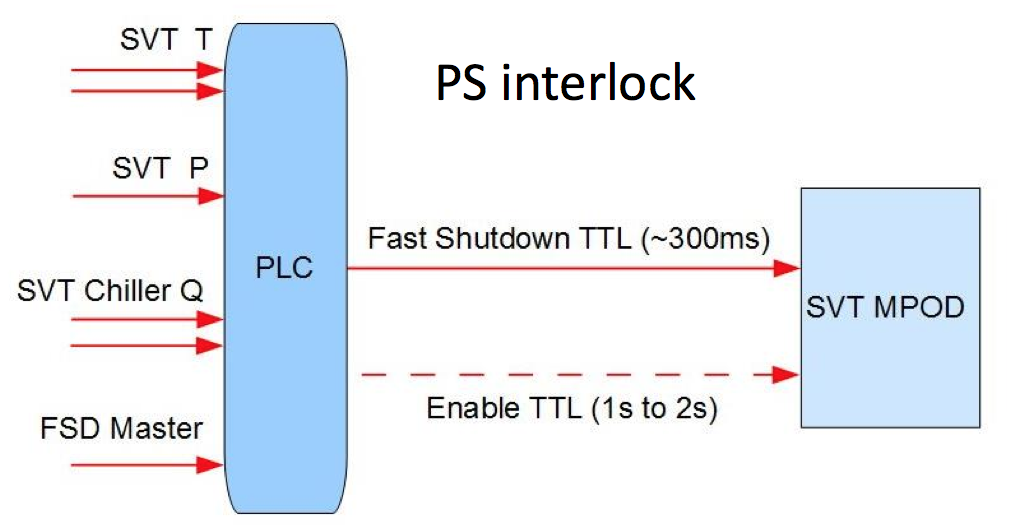
\includegraphics[width=10cm]{svt_interlock_diagram}
\caption{Diagram of the SVT interlocks.\label{fig:svt_interlock_diagram}}
\end{figure}
The interlock system is based on an Allen-Bradley PLC that receives input signals and performs the necessary logic to issue an interlock signal. The interlock signal that triggers a fast shutdown of the SVT power supplies are:
\begin{itemize}
\item Hybrid and front end board temperature
\item Input and output coolant temperature of the SVT hybrid and front end board cooling loops.
\item Coolant fluid pressure in the SVT hybrid and front end board cooling loops.
\item Chiller setting and status of the SVT and hybrid and front end board chillers.
\item Signal from the fast shutdown system of the accelerator. 
\end{itemize}
 Each power control interface (flange board, front-end board, hybrid, bias) shows the status of the interlock signal that allows each system to be powered. 

The solenoid valves are interlocked to mitigate any leaks in the cooling system. 
If the flow meter in either cooling loop detects low flow, the valve at that chiller's outlet closes to prevent coolant from being pumped out of a possible leak in that loop. 
If the vacuum gauge detects a loss of vacuum, both solenoid valves close in case the vacuum loss is due to a coolant leak inside vacuum.

\subsection{Potential accidents}
\subsubsection*{Coolant leakage inside vacuum}
A small leak inside the vacuum will be detected by the vacuum gauges. A large leak will trip the flow switch.
\subsubsection*{Coolant leakage outside vacuum}
A small leak will drain the chiller until its level switch trips, then the flow switch will trip. A large leak will trip the flow switch.
\subsubsection*{Low level in SVT cooling system}
The HFE 7000 fluid is very volatile and is known to evaporate from the chiller reservoir. Any bad seals in the system would increase the rate of loss. The observed rate of loss in testing is less than 1 L/week, and the reservoir capacity is more than 5 L, but the level should be monitored regularly. A low level warning (reported in RS-232 status) will precede a low level alarm (chiller trip).
\subsubsection*{Chiller failure or abnormal operation}
A pump or power failure in a chiller will trip the flow switch.

A refrigerator or control failure may cause the chiller to run at an unexpected temperature. This would be detected by the RTDs.
\subsubsection*{Blockage in a cooling line}
A blockage in the FEB cooling loop, or the SVT cooling lines before the manifold, would reduce total flow in the system. This would be detected by the flow switch or the RTD on the return side.

A blockage in one half of the SVT cooling manifold would reduce flow to half the SVT but might not be detectable by any of the cooling loop instrumentation. The only likely indication is a rise in the SVT hybrid temperatures. Since we don't expect this to happen suddenly or require rapid intervention, we will set an alarm on the SVT hybrid temperatures but no interlock.
\subsubsection*{Beam trip}
The SVT HV must be shut off following a trip, to ensure that the HV is not accidentally left on while the beam is being brought back.

\subsection{Interlocks for operation with beam}
All interlocks are triggered by PLC inputs. Actions are divided into PLC (fast and reliable, since the inputs, logic and outputs are all internal to the PLC) and EPICS (slower, less reliable, less critical)
\subsubsection{Cooling loop failure (high or low temperature on either RTD, or flow switch trip)}
Trip points must be adjustable to allow for operation at different temperatures. There must be some sort of interlock bypass for system startup (i.e. it must be possible to start the chiller when temperatures are out of spec and the flow switch is tripped).
\begin{itemize}
    \item PLC interlock: Close the valve at the chiller outlet. Disable the MPOD.
    \item Software interlock: Turn off the chiller.
\end{itemize}

\subsubsection{Bad vacuum (vacuum gauge)}
\begin{itemize}
    \item PLC and software interlocks: Same action as cooling loop failure, for both loops. (so chillers will be valved off and shut off, and the MPOD will be disabled)
\end{itemize}

\subsubsection{Beam off (BPM signal)}
%There should be an option to have a PLC interlock that disables the MPOD.
If the beam is lost, the SVT should automatically go to a safe configuration until beam is restored.
The specific actions for this interlock depend on how cautious we are being.
\begin{itemize}
\item Software interlock: Turn off all HV channels.
\item Software interlock: Fully retract both SVT positioners.
\end{itemize}


\section{Motion}
\begin{figure}[ht!]
\centering
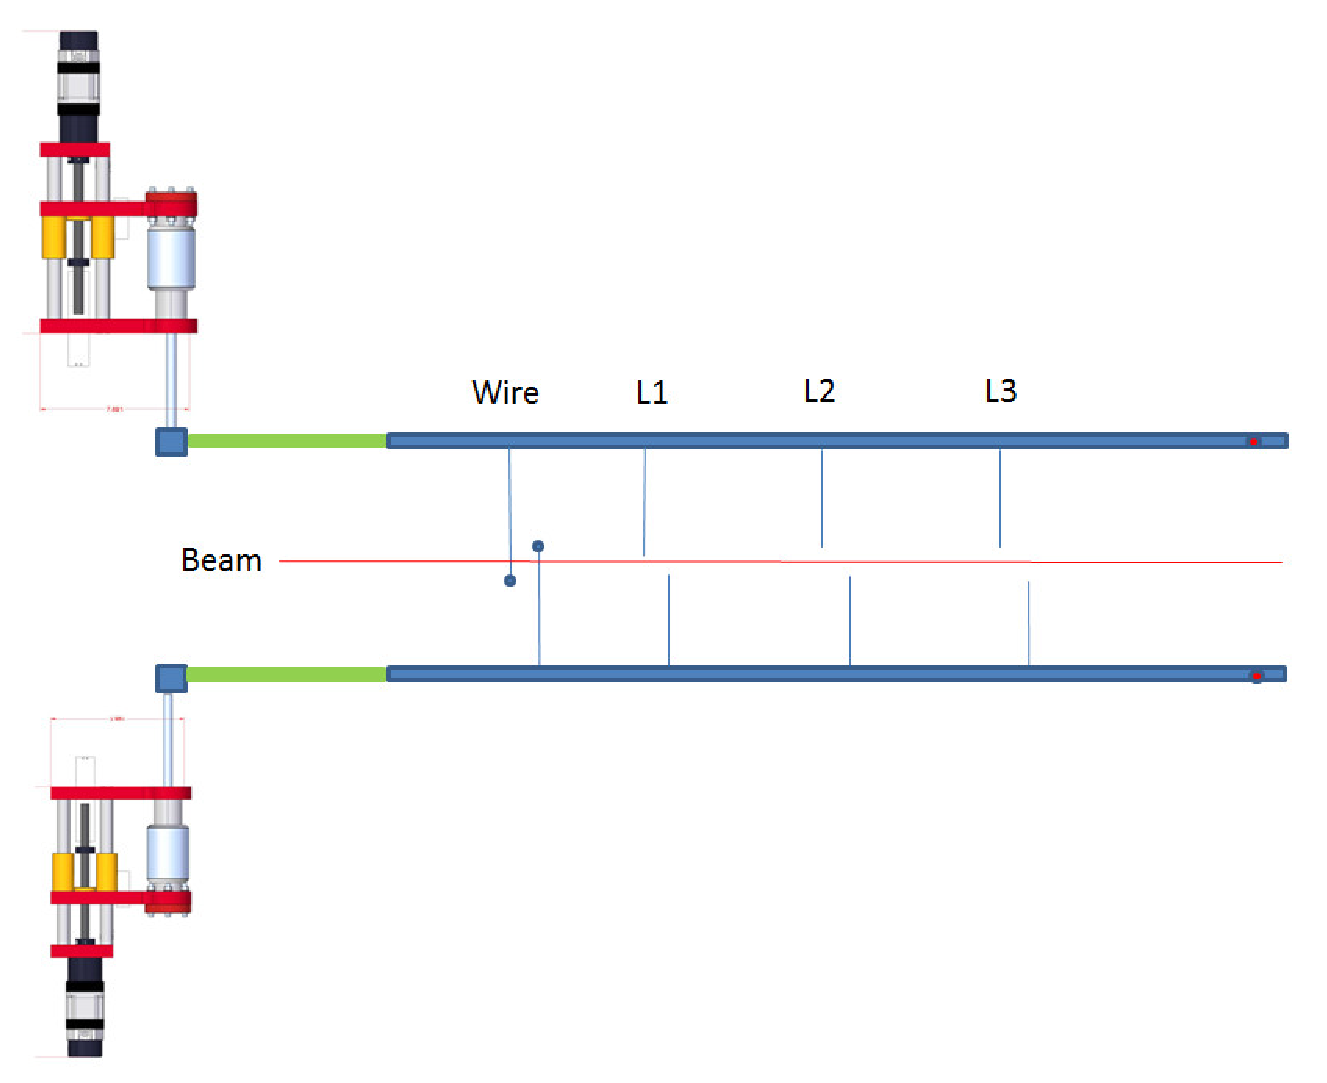
\includegraphics[width=15cm]{motion.eps}
\caption{SVT Motion System}
\label{fig:motion}
\end{figure}

Figure~\ref{fig:motion} shows the SVT Motion System schematically. The top/bottom of each SVT support plate has three sensor layers (L1, L2, L3) and a wire frame, supported on a bearing at one end and connected to a rod attached to a linear stage at the other end. The linear stage is moved by a stepper motor through the EPICS slow controls system. In the nominal run position, the support plates are parallel to the beam and the Silicon physical edge is at 0.5 (L1), 2.0 (L2), and 3.5 mm (L3) from the beam. The support plates can be retracted by 1.3 degrees. Figure~\ref{fig:beam} shows the beam's eye view of the wires and the L1 sensor edge in the nominal run position and in the fully retracted position.

The stepper motor controller is Newport XPS controller, and is different from the stepper motor controllers found in Hall B. The motor control is based on an optical encoder. Stage movement is precisely calibrated, and re-calibration is not necessary. Since the encoder has no knowlege of the actual stage position when the controller power is turned on, the linear stage must move to a reference point to establish its calibration (called ``homing''). A switch is located at the fully retracted position for this purpose. 

Three vertical coordinates are used to locate the stage, the horizontal wire and the layer 1 sensor physical edge. The stage coordinate is y(stage) = 0 mm at the fully retracted position and y(stage) = 18.89 mm at the nominal run position for both top and bottom stages. The wire and sensor edge coordinates are measured relative to the nominal beam position (positive y is up), and are given in terms of y(stage) as,

\begin{itemize}
\item
y(top-wire) = -0.482 $\cdot$ y(stage) + 1.76 mm,
\item
y(top-si) = -0.391 $\cdot$ y(stage) + 7.89 mm,
\item
y(bottom-wire) = +0.463 $\cdot$ y(stage) - 1.39 mm,
\item
y(bottom-si) = +0.372 $\cdot$ y(stage) - 7.53 mm.
\end{itemize}

As the coordinate transformation is done automatically, all you need to specify is the position of the wire or Si sensor edge to operate the SVT Mover and the SVT Wire Scanner. 

\begin{figure}[ht!]
\centering
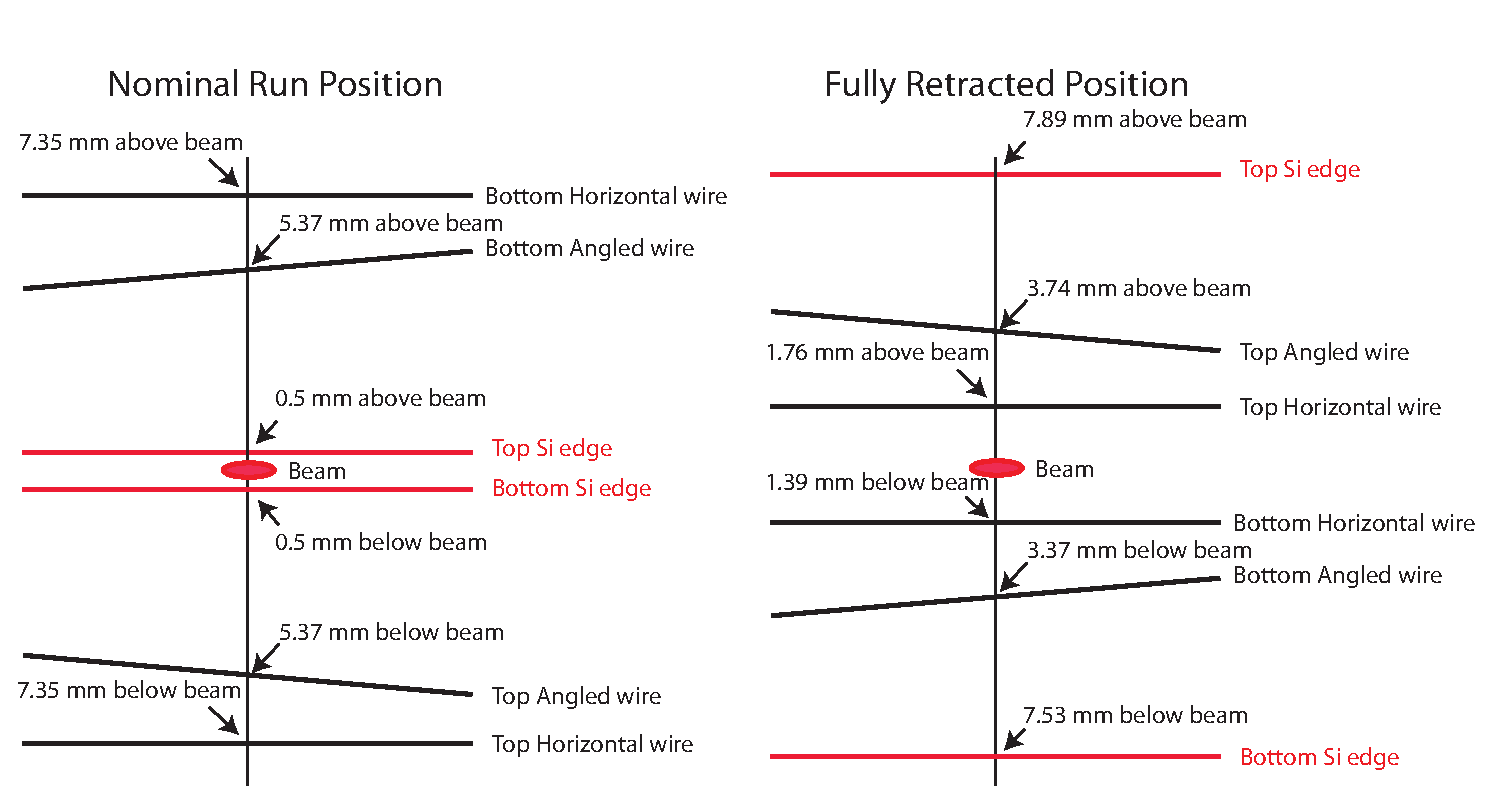
\includegraphics[width=15cm]{WireFrame2.eps}
\caption{Beam's eye view of wires and and L1 sensor edge}
\label{fig:beam}
\end{figure}




\chapter{Controls and monitoring}

\section{Voltages}
\label{sec:monitoring_power}
The SVT power and bias as well as alarms are monitored through several GUI's. All GUI's are accessible from the main HPS control screen. To start it:

\begin{enumerate}
\item Log into the \textbf{clonioc1} computer in the counting house.

\begin{figure}[ht!]
\centering
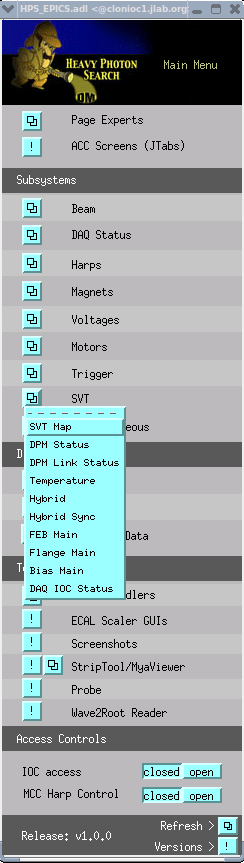
\includegraphics[width=3cm]{epics_dev_svt.png}
\caption{HPS EPICS main GUI. \label{fig:hps_epics_svt}}
\end{figure}

\item Open a terminal and issue \texttt{hps\_epics dev} command to open the main HPS GUI. Figure~\ref{fig:hps_epics_svt} show the SVT part of the GUI open.
\item Each of the individual GUIs can be opened by clicking the appropriate button in the HPS main GUI that opened.
\end{enumerate}

Below is a description of each of the GUI's in the list.

\begin{figure}[ht!]
\centering
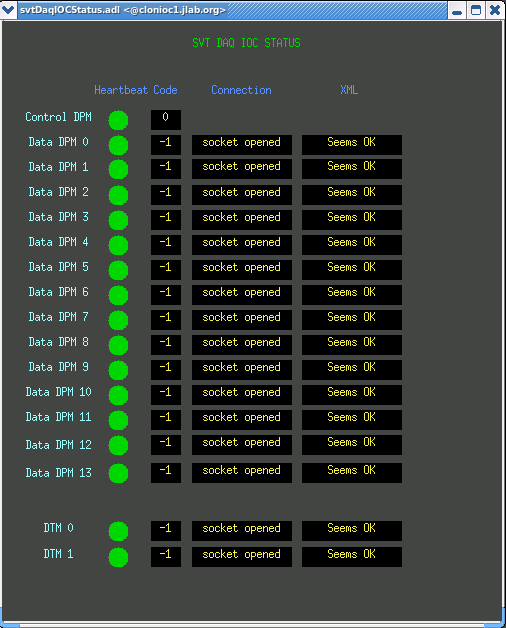
\includegraphics[width=8cm]{svtDaqIOCStatus.png}
\caption{DAQ IOC Status GUI. \label{fig:svtDaqIOCStatus}}
\end{figure}

\begin{itemize}
\item \textbf{DAQ IOC Status} in Fig.~\ref{fig:svtDaqIOCStatus}.
\begin{itemize}
\item Monitoring: status and error codes from all SVT DAQ IOCs.
\end{itemize}

\item \textbf{DPM Status} in Fig.~\ref{fig:svtDpmStatus}.
\begin{itemize}
\item Monitoring: run state and event counts  from the data processing nodes in the SVT DAQ.
\end{itemize}

\begin{figure}[ht!]
\centering
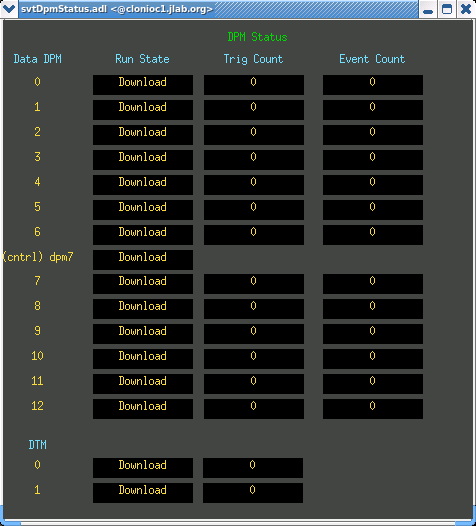
\includegraphics[width=8cm]{svtDpmStatus.png}
\caption{DPM state GUI. \label{fig:svtDpmStatus}}
\end{figure}

\begin{figure}[hb!]
\centering
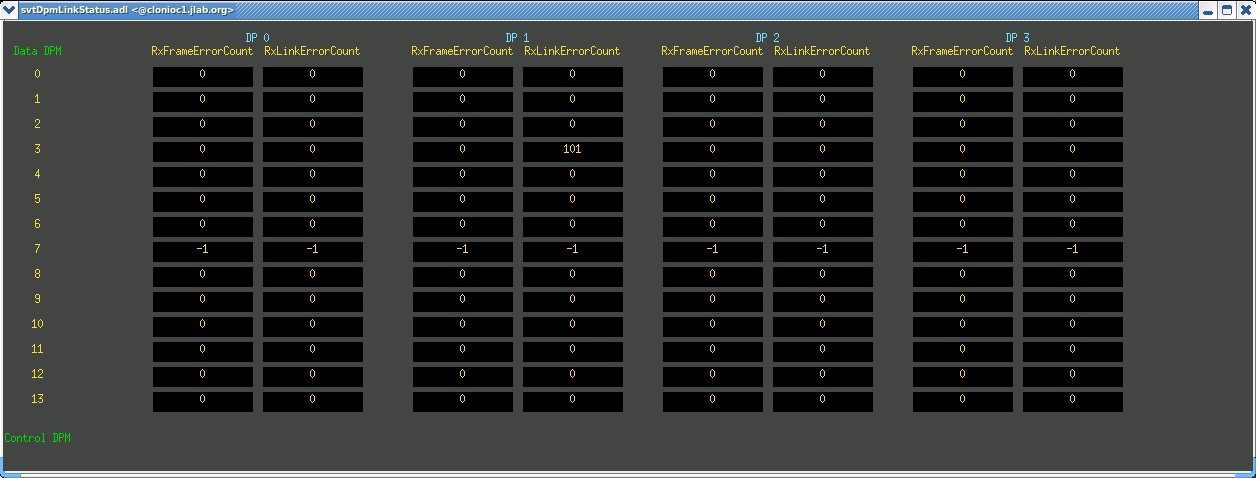
\includegraphics[width=13cm]{svtDpmLinkStatus.png}
\caption{DPM link status GUI. \label{fig:svtDpmLinkStatus}}
\end{figure}

\item \textbf{DPM  Link Status} in Fig.~\ref{fig:svtDpmLinkStatus}.
\begin{itemize}
\item Monitoring: link errors for each of the data processing nodes in the SVT DAQ.
\end{itemize}

\item \textbf{Temperature} in Fig.~\ref{fig:svtTemp}.
\begin{itemize}
\item Monitoring: FEB (3 temperatures), 
\item Monitoring: FEB cooling temperature on the supply and return at the PS magnet for the FEB and SVT chiller.
\end{itemize}

\item \textbf{Hybrid GUI} in Fig.~\ref{fig:svtHybrid}.
\begin{itemize}
\item Monitoring: all measured voltage and currents from hybrids. 
\item Monitoring: temperature from hybrids. 
\item Control: ON/OFF switch for each of the three voltages for individual hybrids and all hybrids.
\end{itemize}

\begin{figure}[ht!]
\centering
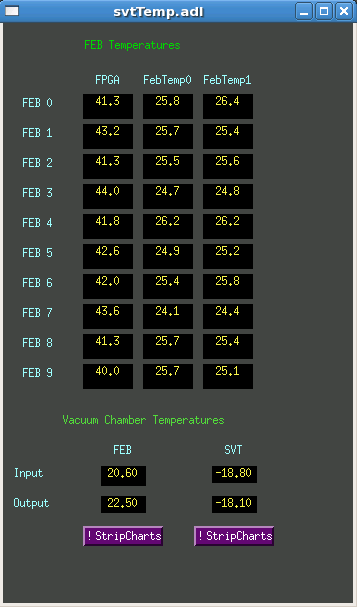
\includegraphics[width=5cm]{svtTemp.png}
\caption{Temperature GUI. \label{fig:svtTemp}}
\end{figure}

\begin{figure}[hb!]
\centering
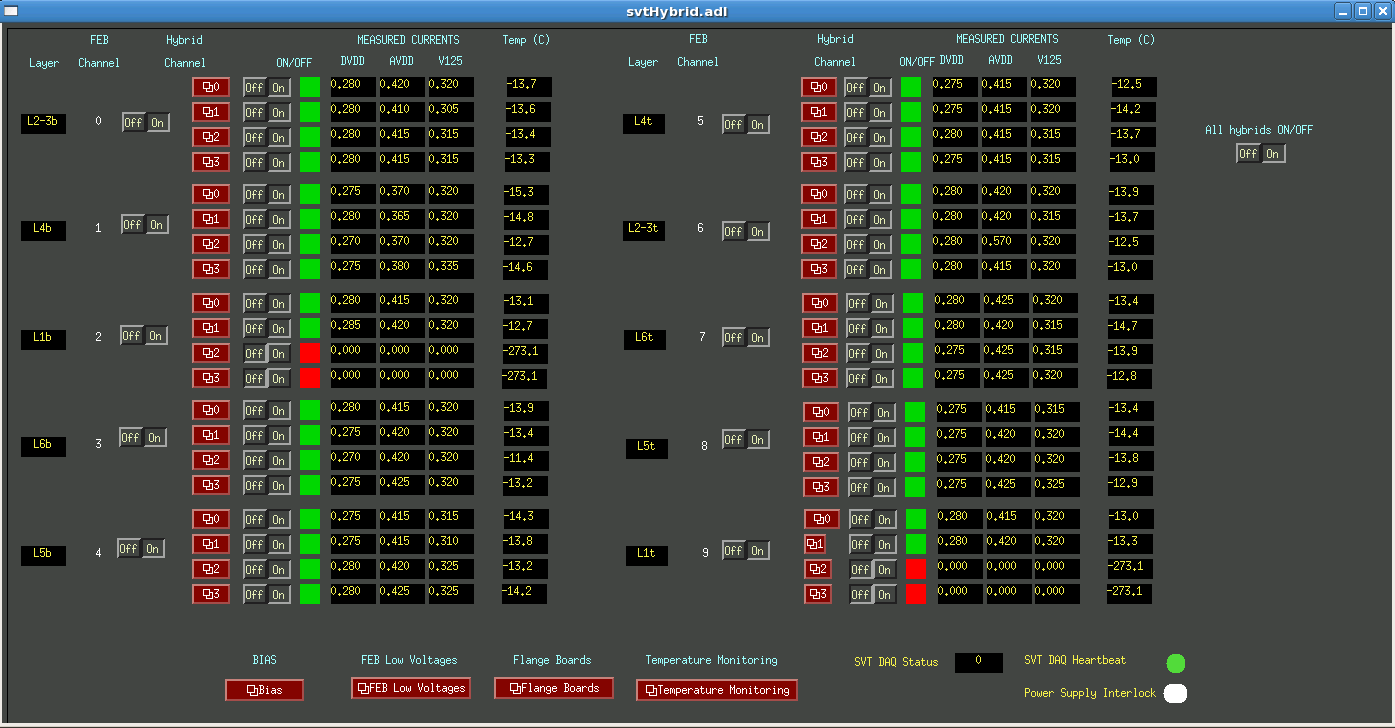
\includegraphics[width=13cm]{svtHybrid.png}
\caption{Hybrid power and temperature GUI. \label{fig:svtHybrid}}
\end{figure}

\item \textbf{Hybrid Sync} in Fig.~\ref{fig:svtHybridSync}.
\begin{itemize}
\item Monitoring: sync status for each hybrid.
\item Monitoring: base and peak value of the sync pulse from each hybrid. (EXPERT ONLY). 
\end{itemize}

\begin{figure}[ht!]
\centering
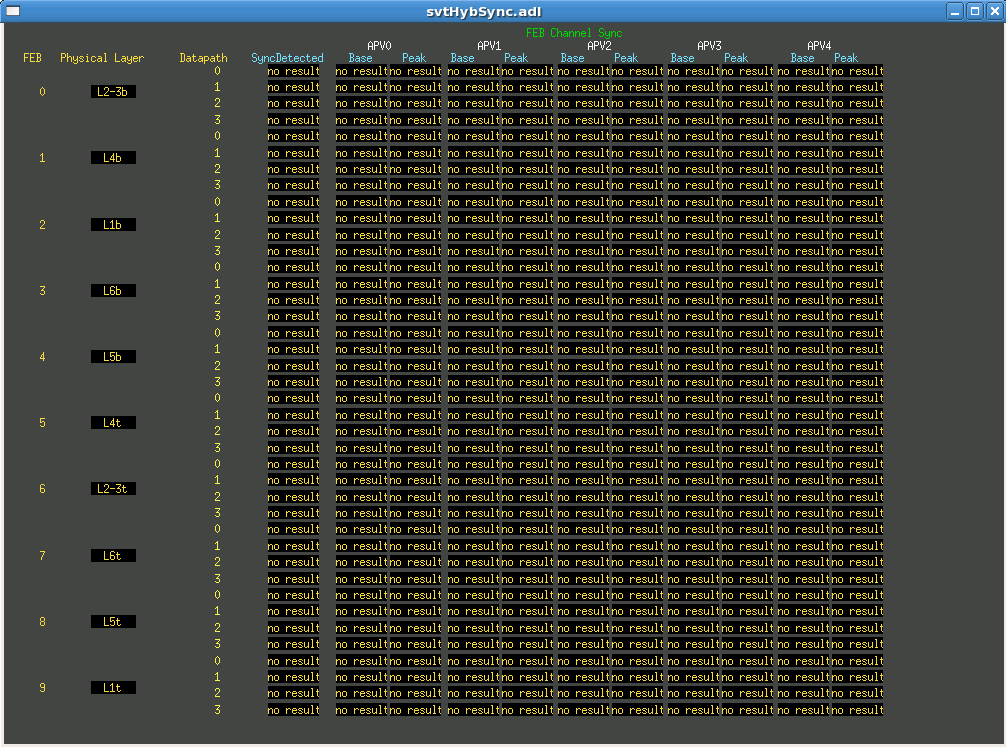
\includegraphics[width=14cm]{svtHybridSync.png}
\caption{Hybrid sync GUI. \label{fig:svtHybridSync}}
\end{figure}

\item \textbf{FEB Power GUI} in Fig.~\ref{fig:svtFebMain}.
\begin{itemize}
\item Monitoring: all currents and voltages of the FEB.
\item Control: ON/OFF switch for all FEB boards. 
\item Control: ON/OFF switch for each FEB board. 
\item Control: Set point for voltage, trip and ramp values for each flange board (EXPERT ONLY).
\end{itemize}

\item \textbf{Flange power GUI} in Fig.~\ref{fig:svtFlange}.
\begin{itemize}
\item Monitoring: all  currents to the flange boards. 
\item Control: ON/OFF switch for all flange boards. 
\item Control: ON/OFF switch for each flange board. 
\item Control: Set point for voltage, trip and ramp values for each flange board (EXPERT ONLY).
\end{itemize}

\item \textbf{High voltage bias GUI} in Fig.~\ref{fig:svtBias}.
\begin{itemize}
\item Monitoring: all voltage set points for the SVT sensors.
\item Control: ON/OFF switch for all sensors.
\item Control: ON/OFF switch for each sensor.
\item Control: Set point for voltage for all modules (EXPERT ONLY).
\item Control: Set point for voltage and ramp values for each module (EXPERT ONLY).
\item Control: \textbf{RESET INTERLOCKS} button to restore normal function after an MPOD trip.
\end{itemize}



\end{itemize}

\begin{figure}[h!t]
\centering
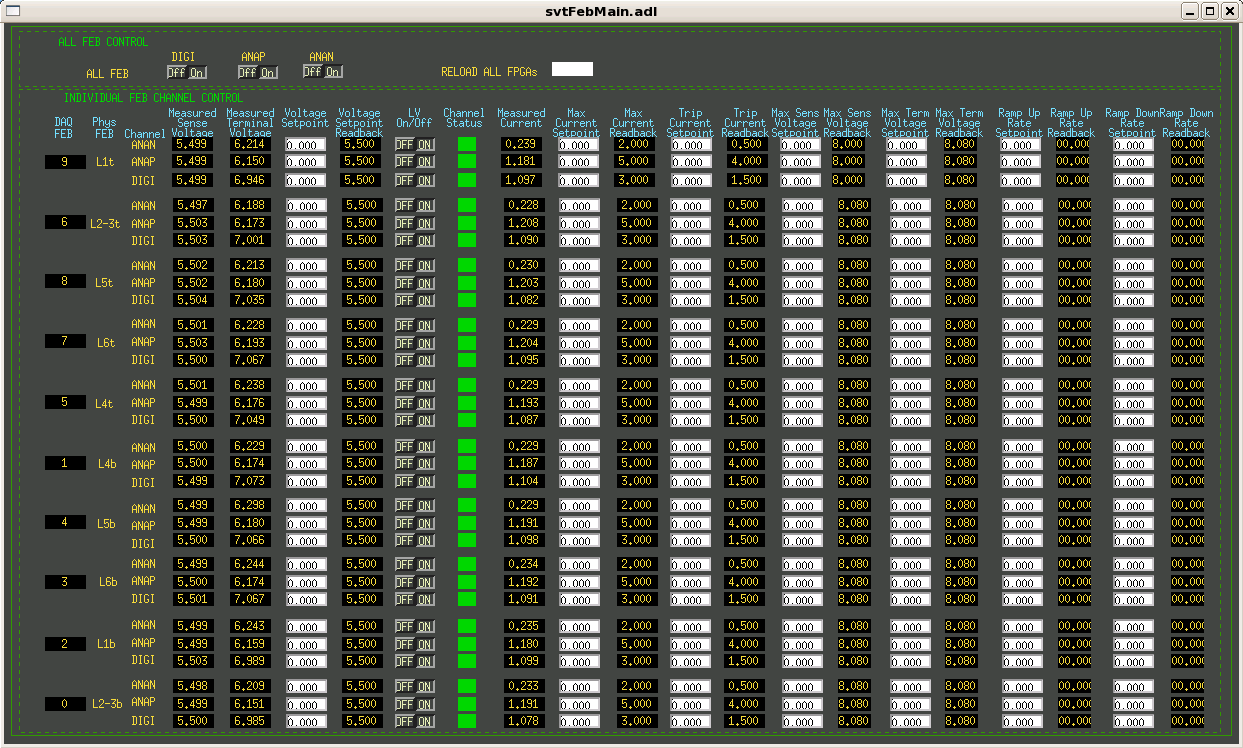
\includegraphics[width=14cm]{svtFebMain.png}
\caption{FEB power GUI. \label{fig:svtFebMain}}
\end{figure}

\begin{figure}[h!t]
\centering
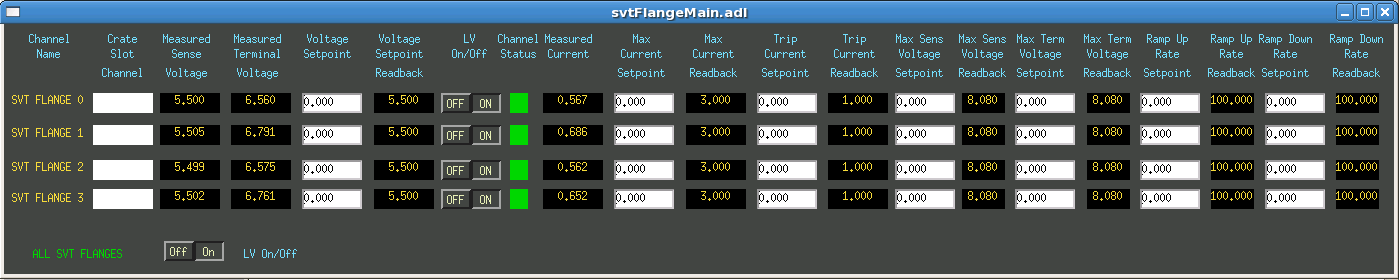
\includegraphics[width=14cm]{svtFlange.png}
\caption{Flange power GUI. \label{fig:svtFlange}}
\end{figure}

\begin{figure}[h!]
\centering
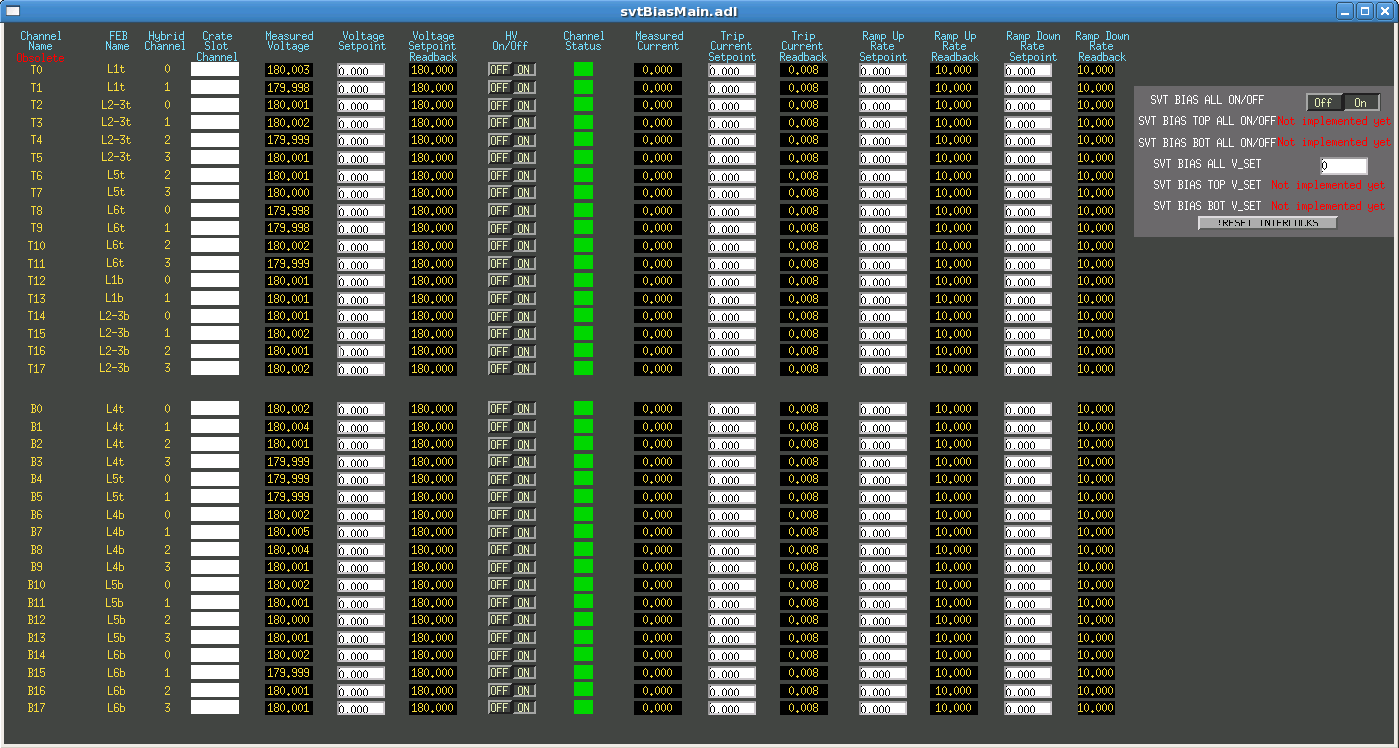
\includegraphics[width=14cm]{svtBias.png}
\caption{High voltage bias GUI. \label{fig:svtBias}}
\end{figure}

\section{SVT Cooling}

All the GUIs shown below are accessed through the \textbf{Devices} menu in \textbf{hps\_epics}. Chiller and interlock settings should only be modified under the supervision of an SVT Expert. Table~\ref{tab:cooling_settings} lists the default settings for the SVT and FEB chillers and alarms during running (cold) and between runs when the beam enclosure is open for servicing (warm).

\begin{figure*}[!ht]
    \begin{center}
        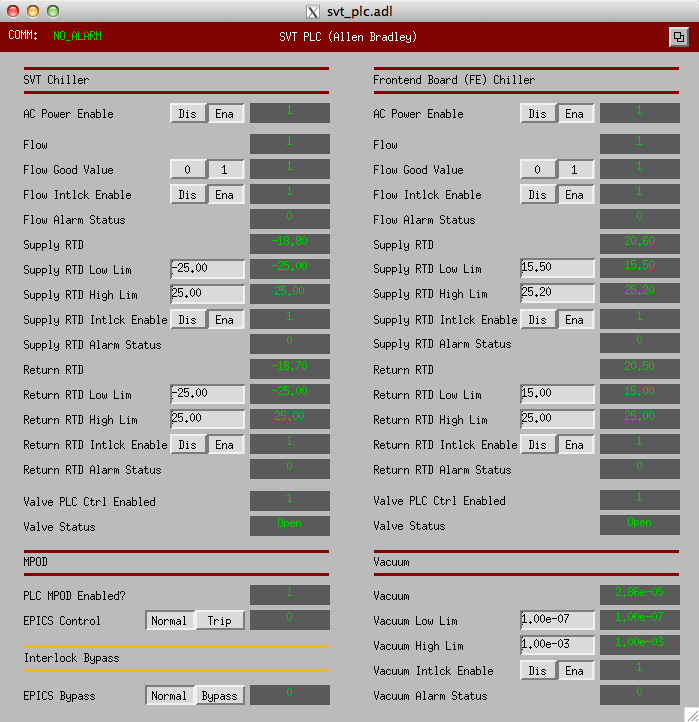
\includegraphics[width=0.5\textwidth]{svt_plc.png}
        \caption{SVT PLC GUI, accessed through the \textbf{Devices} menu in \textbf{hps\_epics}.}
        \label{fig:ctrl_cooling_plc}
    \end{center}
\end{figure*}

\begin{figure*}[!ht]
    \begin{center}
        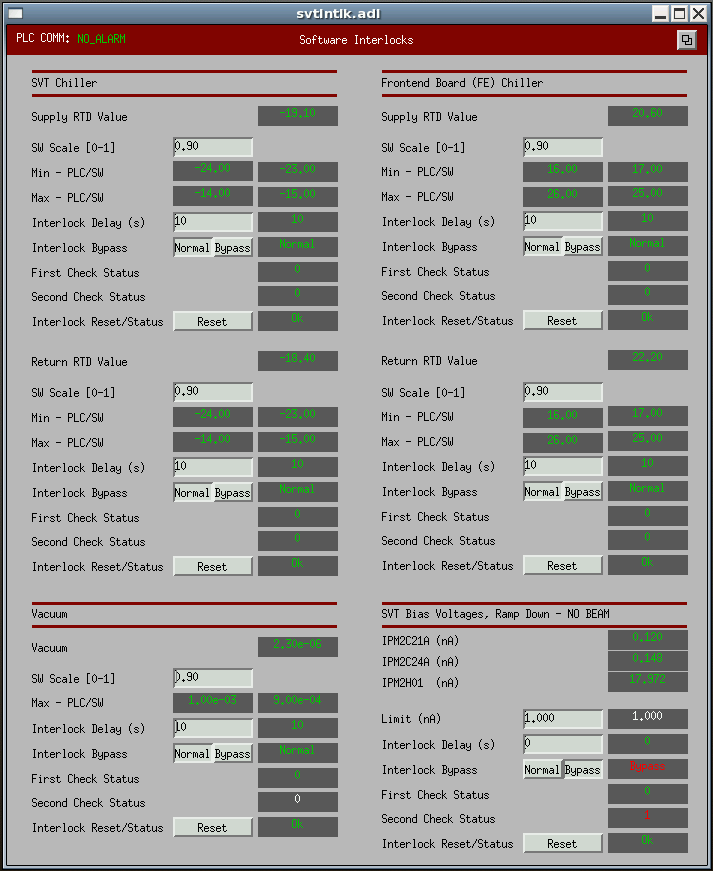
\includegraphics[width=0.4\textwidth]{svt_softinterlocks.png}
        \caption{SVT software interlocks GUI, accessed through the \textbf{Devices} menu in \textbf{hps\_epics}.}
        \label{fig:ctrl_cooling_softinterlocks}
    \end{center}
\end{figure*}

\begin{figure*}[!ht]
    \begin{center}
        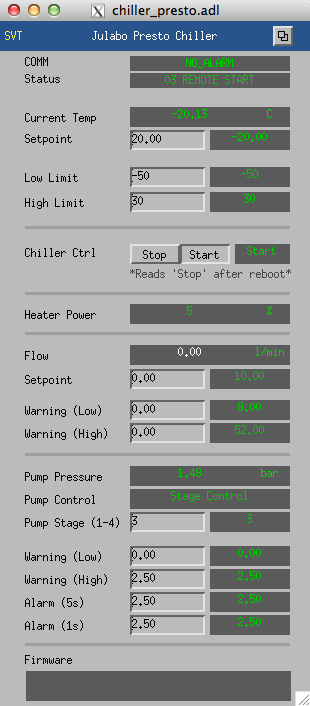
\includegraphics[width=4cm]{figures/svt_svtChiller.png}
        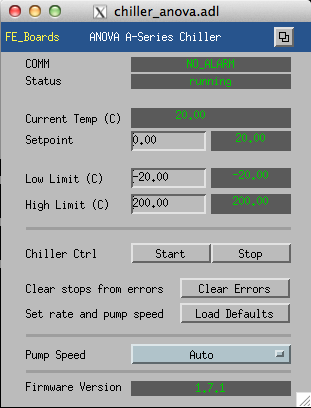
\includegraphics[width=0.3\textwidth]{figures/svt_febChiller.png}
        \caption{SVT (left) and FEB (right) chiller GUIs, accessed through the \textbf{Devices} menu in \textbf{hps\_epics}.}
        \label{fig:ctrl_cooling_chillers}
    \end{center}
\end{figure*}

\begin{table}[h]
\begin{center}
\begin{tabular}{|l|l|l|}
\hline
Parameter & SVT warm & SVT cold \\
\hline
SVT chiller setpoint ($^\circ$C) & 17 & -20 \\
SVT RTD alarms (\textbf{{\color{red} low}/{\color{yellow} low}/{\color{yellow}high}/{\color{red}high}}) ($^\circ$C) & \textbf{{\color{red}15}/{\color{yellow}16}/{\color{yellow}18}/{\color{red}19}} & \textbf{{\color{red}-22}/{\color{yellow}-21}/{\color{yellow}-17}/{\color{red}-16}} \\
SVT RTD PLC limits ($^\circ$C) & bypassed & -24/-14 \\
FEB chiller setpoint ($^\circ$C) & 20 & 20 \\
FEB RTD alarms (\textbf{{\color{red} low}/{\color{yellow} low}/{\color{yellow}high}/{\color{red}high}}) ($^\circ$C) & \textbf{{\color{red}16}/{\color{yellow}17}/{\color{yellow}25}/{\color{red}26}} & \textbf{{\color{red}16}/{\color{yellow}17}/{\color{yellow}25}/{\color{red}26}} \\
FEB RTD PLC limits ($^\circ$C) & bypassed & 16/26 \\
\hline
\end{tabular}
\end{center}
\caption{Default SVT cooling settings.  Minor alarm limits are in yellow and major alarm limits are in red.}
\label{tab:cooling_settings} 
\end{table}

Any major (red) ALH alarm under the ``SVT/COOLING'' group will send an e-mail alert. Also, there is a webcam (cctv7) pointed at the SVT chiller screen. The webcam can be set to e-mail a snapshot every 24 hours. 

\section{Motion}

The SVT movers are controlled using the SVT positioner GUI.
The GUI controls the top and bottom halves of the SVT separately.
For each half, the GUI shows the position in four ways: stage position, wire-to-beam distance, layer-1-to-beam distance, and angle. Except for the stage position (0 at home, positve as the stage moves in), these are signed values (positive above the beamline, negative under it).

\begin{figure}[h!t!]
\centering
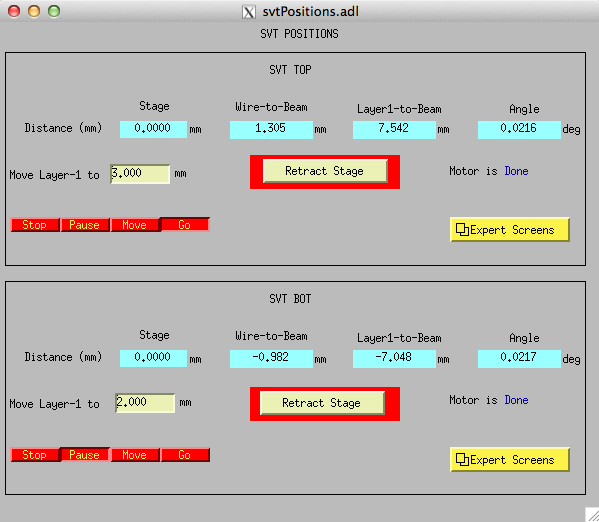
\includegraphics[width=8cm]{svt_movers.png}
\caption{SVT positioner GUI, accessed through the \textbf{Motors} menu in \textbf{hps\_epics}.}
\label{mover}
\end{figure}


The \textbf{Retract Stage} button moves the stage to 0.000 (all the way out).
The button is disabled (red border) if this half of the SVT is already all the way out.

The \textbf{Move Layer-1 to} text box moves the SVT to user-defined positions.
Type the desired (signed) value of the layer-1 distance and press \textbf{Enter} to move the stage.
There is a software limit (a minimum layer-1 distance) to prevent unsafe operation of the SVT; the limit is not displayed on this GUI but should be listed in the shift instructions.

\emph{Sometimes there is no response to an input in the text box. If this happens, one workaround is to open the motor expert GUI (click the \textbf{Expert Screens} button), and enter a value in either \textbf{MoveAbs} field. This seems to kick the motor control out of whatever bad state it gets stuck in.}



\section {Online Monitoring}

The SVT will be monitored online using the Java based HPS Monitoring Application.
The most basic set of plots can be brough up by issuing the following commands 
from a terminal:  

\begin {itemize}
    \item Log into \textbf{clonpc19} in the counting house as \texttt{hpsrun}
    \item Open a terminal and navigate to \texttt{/home/hpsrun/svt\_monitoring}
    \item Issue the command \texttt{python run\_svt\_monitoring.py} to open the monitoring app
\end {itemize}
Pressing the connect button will bring up plots SVT occupancies, raw hit counts
and raw hit ADC sample amplitudes.  Once a run had ended, the plots need to be 
brough down manually.

\subsection {Occupancies}

\begin{figure}[h!]
    \centering
    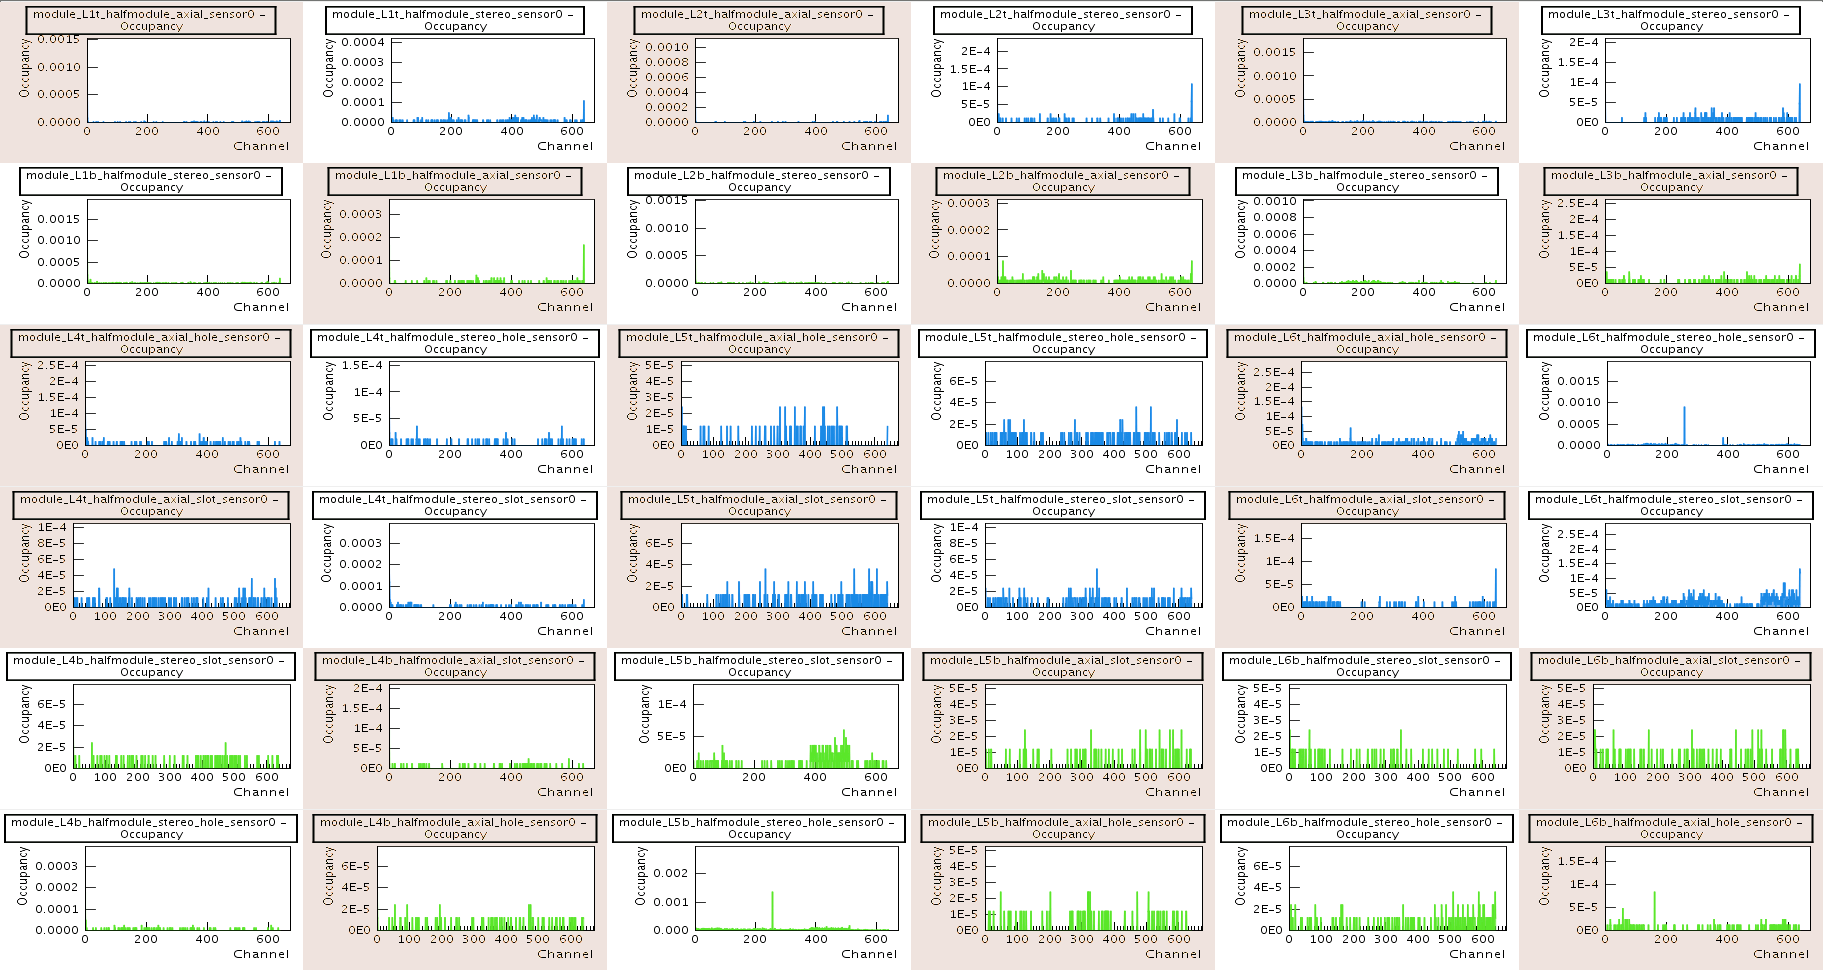
\includegraphics[width=\textwidth]{figures/occupancy_monitoring_app.png}
    \caption{SVT occupancies plot.}
    \label{fig:occupancies}
\end{figure}

\subsection {SVT Hits}

\subsection {Samples}





\chapter{Procedures}


\section{General Procedures}
\subsection{Checklist: Preparing for beam}
\label{sec:proc_general_beamchecklist}
This verifies that the SVT is ready for beam. This checklist should be done before any beam passes through HPS.
\begin{enumerate}
\item Check that the chillers are running.
\item Check the interlocks.
\item Check that voltages are on.
\item Check the SVT soft limits: Open the SVT positioner GUI. For each half of the SVT, open the \textbf{Motor Expert Gui} (under \textbf{Expert Screens}) and check the \textbf{Hi limit} against the shift instructions.
%\item Check the SVT shift instructions for ``Before Beam'' settings.
\item Set the beam interlock: {\color{red} doesn't exist yet}
\end{enumerate}

\subsection{Starting a run with beam}
\label{sec:proc_general_startrun}
\begin{enumerate}
\item Reset the beam interlock: go to the SVT software interlocks GUI, push the \textbf{Bypass} button, the \textbf{Reset} button, then the \textbf{Normal} button.
\item To close the SVT (if the motion interlock was enabled): open the SVT positioner GUI.
For each half of the SVT, type the required position (see shift instructions) in the \textbf{Move Layer-1 to} box and hit \textbf{Enter}.
Verify that the positions shown in the scaler GUI match the required position.
\item To turn on HV (if the HV interlock was enabled): follow the \textbf{Turn on SVT High Voltage Bias} portion of the \textbf{Turning the SVT power and bias ON} procedure, \ref{sec:proc_voltages_allon}.
\item If the run was stopped: start the run (see the DAQ manual).
\end{enumerate}

\subsection{Response to beam trip}
\label{sec:proc_general_beamtrip}
If the beam is lost, the SVT software interlock may (depending on settings) turn off all HV channels or open the SVT.

\begin{enumerate}
\item Check the SVT shift instructions to see what actions are required.
\item {\color{red} What should be checked for DAQ?}
\item If the HV interlock was enabled: Look at the SVT bias GUI, and verify that the \textbf{Measured Voltage} column reads 0 for all channels. If not, call the expert. Continue with the procedure.
\item If the motion interlock was enabled: Look at the scaler GUI, and verify that the \textbf{Position} of the top and bottom read 0.0000.
\item If the run needs to be stopped, see the DAQ manual for instructions.
\item Wait for good beam to be restored, then follow the procedure for starting a run, \ref{sec:proc_general_startrun}.
\end{enumerate}

\section{Response to Alarms}

The alarm handling is handled by the ALH extension to EPICS that is widely used at JLab. The SVT alarm handling GUI is shown in Fig.~\ref{fig:svt_alarm_gui}. It is tree-based with each level showing more detailed info of what alarm has gone off. 
\begin{figure}
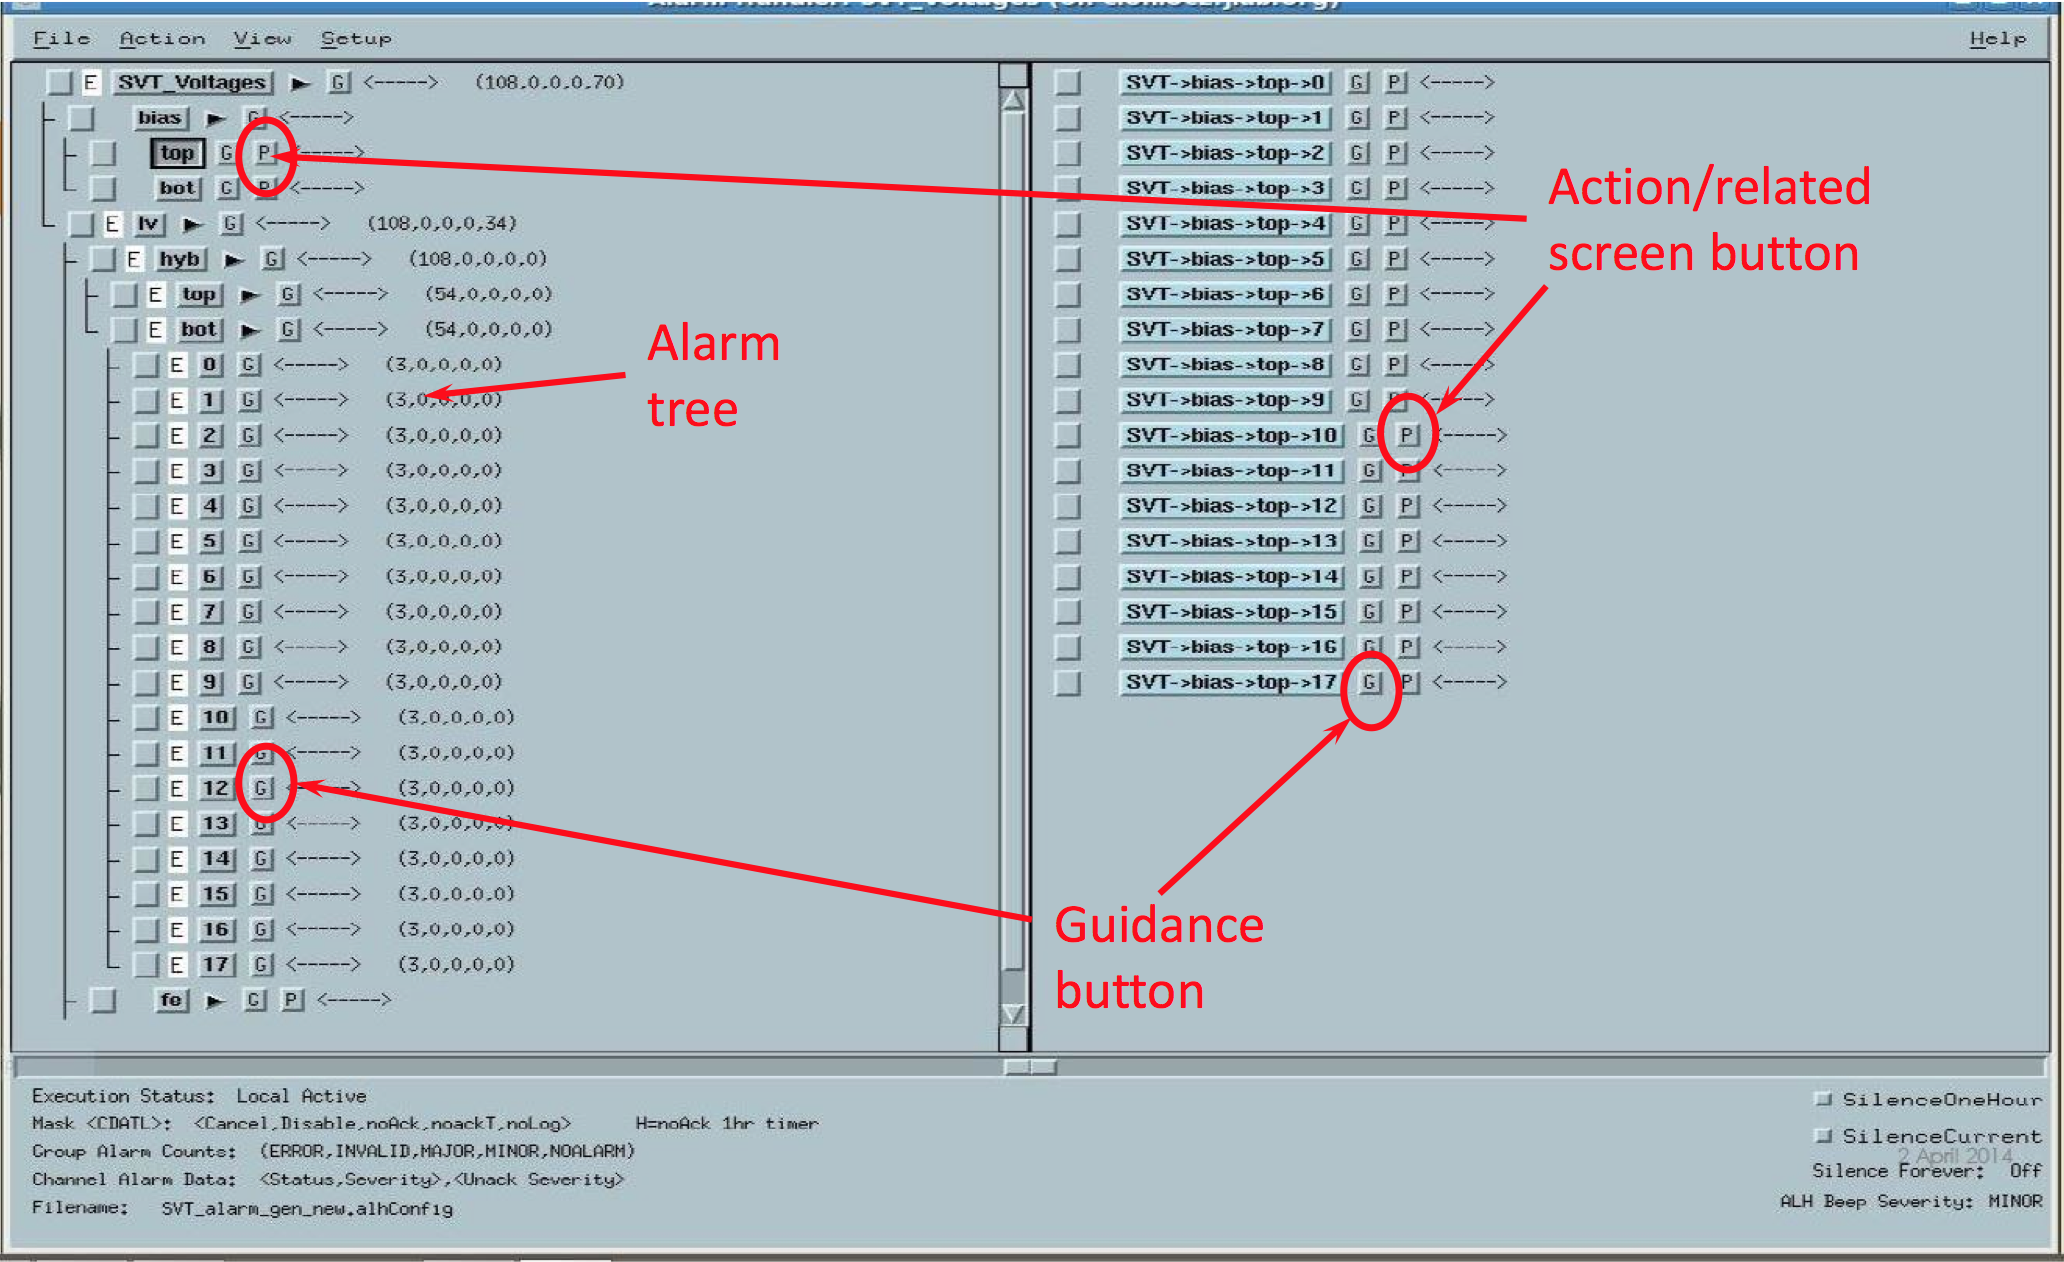
\includegraphics[width=12cm]{svt_alarm_gui}
\caption{SVT alarm handler GUI.\label{fig:svt_alarm_gui}}
\end{figure}

Each level has two buttons: a \textbf{guidance} button which opens a pop up display with more information and an \textbf{action} button which acknowledges the alarm. 

\begin{verbatim}
In case any error please contact SVT expert.
\end{verbatim}
\begin{verbatim}
Be ready to report what alarm has gone off.
\end{verbatim}

More information about the alarm handler can be found in the slow control manual. 


\section{Voltages}
\label{sec:proc_voltages}
\subsection{Turning the SVT power and bias ON}
\label{sec:proc_voltages_allon}
To power ON all of the SVT follow this procedure:
\begin{enumerate}

\item Turn on SVT FEB Power
\begin{enumerate}
\item 
Make sure that the SVT and FEB chillers are \textbf{ON} and \textbf{OK}, and the PLC interlock is enabled and OK. See Sec.~\ref{sec:proc_cooling} for operation of the cooling system.
\item
The flange power should be OFF. Go to the flange power GUI and turn if OFF (see below) .
\item
Open the the FEB Power GUI (svtFebMain.adl) shown in Fig.~\ref{fig:svtFebMain}. See~\ref{sec:monitoring_power} to restart GUI if not running.
\item
At the top of the GUI: press the \textbf{On} switch marked \textbf{DIGI}. Wait until the corresponding channel status indicator turns \textbf{GREEN} for all ten FEBs. 
\item
Repeat for \textbf{ANAP} and \textbf{ANAN}.
\end{enumerate}


\item Turn on SVT Flange Power
\begin{enumerate}
\item
Open the SVT Flange Power Control GUI, see Fig.~\ref{fig:svtFlange}  (see~\ref{sec:monitoring_power} to restart if not running).
\item
Press the \textbf{ON} switch for the \textbf{ALL SVT FLANGES} section at the bottom of the GUI. Wait until the status indicator turns {\color{green} \textbf{GREEN}}  for every one of the four flange boards, and check for alarms after currents stabilized. 
\end{enumerate}



\item Checklist  that FEBs are powered correctly:
\begin{enumerate}
\item
Open the SVT DAQ IOC Status GUI (svtDaqIOCStatus.adl) and check that all IOC report OK status.
\item
Open the SVT temperature GUI (svtTemp.adl) and check that all 10 FEB show reasonable temperatures and that they are updating about every second.
\item
Open the DPM Link Status GUI (svtDpmLinkStatus.adl) and look for incrementing counters on any of the columns. \newline 
If there is a DPM that has a rate larger than one per minute recycle, try to recycle the flange power (waiting 10s before turning on again). You may need to recycle this up to four times.
\end{enumerate}





\item Turn on SVT Hybrid Power
\begin{enumerate}
\item
Make sure the FEBs and flange are powered and OK following the above procedure.
\item 
Find the SVT Hybrid GUI (svtHybrid.adl) in Fig.~\ref{fig:svtHybrid}.
Wait until all status indicators turn \textbf{GREEN}, currents are seen updating and no alarms go off.\newline
NOTE: at this time this might take up to 1minute during which the SVT DAQ GUIs may be in a bad state. If it takes more than 1 minute call the SVT expert.
\item
Check hybrids currents and temperatures are within range and no alarms go off.
\end{enumerate}





\item Turn on SVT High Voltage Bias
\begin{enumerate}
\item
Make sure that beam conditions and SVT position has granted permission to turn on HV. \textbf{ask the shift leader if you are not sure}.
\item
Find the SVT High Voltage Bias Control GUI (svtBiasMain.adl) shown in Fig.~\ref{fig:svtBias} (see~\ref{sec:monitoring_power} to restart if not running).
\item
Check that the \textbf{Voltage Setpoint Readback} column reads 180V for every channel. If not, call the SVT expert.
\item
Press the \textbf{On} switch marked \textbf{SVT BIAS ALL ON/OFF}.
\item
Wait until all status indicators turn {\color{green} \textbf{GREEN}} and no alarms go off.
\end{enumerate}


\end{enumerate}

\subsection{Turning the SVT power and bias OFF}
\label{sec:proc_voltages_alloff}
To power OFF all of the SVT follow this procedure:
\begin{enumerate}
\item Turn off SVT FEB Power
\begin{enumerate}
\item 
Make sure that the SVT and FEB chillers are \textbf{ON} and \textbf{OK}, and the PLC interlock is enabled and OK. See Sec.~\ref{sec:proc_cooling} for operation of the cooling system.
\item
Find the SVT FEB Power Control GUI shown in Fig.~\ref{fig:svtFebMain} (see~\ref{sec:monitoring_power} to restart if not running)
\item
In the \textbf{ALL FEB CONTROL} section at the top, press the three \textbf{Off} switches marked \textbf{DIGI}, \textbf{ANAP} and \textbf{ANAN}.
Wait until all status indicators turn \textbf{RED} for every one of the ten FEBs, and no alarms go off.
\end{enumerate}

\item Turn off SVT Flange Power
\begin{enumerate}
\item
Find the SVT Flange Power Control GUI, see Fig.~\ref{fig:svtFlange}  (see~\ref{sec:monitoring_power} to restart if not running).
\item
In the \textbf{ALL SVT FLANGES} section at the bottom, press the \textbf{Off} switch.
Wait until the status indicator turns \textbf{RED} for every one of the four flange boards, and no alarms go off.
\item
Check that currents are within range (see Sec.~\ref{sec:svt_power_monitoring_alarm_interlocks} below). If not, follow the procedure outlined in that section.
\end{enumerate}

\item Turn off SVT High Voltage Bias
\begin{enumerate}
\item
Find the SVT High Voltage Bias Control GUI shown in Fig.~\ref{fig:svtBias} (see~\ref{sec:monitoring_power} to restart if not running).
\item
Press the \textbf{Off} switch marked \textbf{SVT BIAS ALL ON/OFF}.
\item
Wait until all status indicators turn \textbf{RED} and the \textbf{Measured Voltage} column reads 0V for evey channel, and no alarms go off.
If not, call the SVT expert.
\end{enumerate}

\end{enumerate}

\section{Cooling and Interlocks}
\label{sec:proc_cooling}
\subsection{Start FEB chiller}
\begin{enumerate}
    \item Disable the PLC interlock for FEB flow (PLC GUI, upper right).
    \item Verify that the chiller temperature setpoint is 20 C. If not, call the SVT expert.
    \item Check the RTD temperature limits. The low limits should be set at 16 C and the high limits at 26 C.
    \item Verify that all PLC alarms that affect the FEB chiller loop (supply RTD, return RTD, and vacuum) are in ``0'' state.
    \item Verify that the FEB valve is open.
    \item Start the chiller.
    \item Wait for the flow switch value to change, then enable the FEB flow interlock.
        If the flow switch does not trigger, call the SVT expert.
    \item At this point, the FEBs can be powered.
    \item The \textbf{current temperature} shown in the FEB chiller GUI should converge to the setpoint in a few minutes.
    \item When the temperature has reached the setpoint, lower the high limits in the interlock to their final values.
\end{enumerate}

\subsection{Start SVT chiller}
\begin{enumerate}
    \item Change the chiller temperature setpoint to 17 C. (This assumes the SVT cooling loop is at room temperature to start. If it is cold, start cold.)
    \item Disable the PLC interlocks for SVT flow, supply RTD, and return RTD (left side of PLC GUI).
        Disable the software interlocks for supply RTD and return RTD (left side of software interlock GUI).
        Verify all PLC alarms and software interlocks are in ``Ok'' or ``0'' state, and the SVT valve is open (PLC GUI).
    \item Start the chiller.
    \item Wait for the flow switch value to change, then enable the SVT flow interlock.
    \item Wait for the chiller temperature to stabilize at the setpoint.
        Some oscillation is normal in the short term, and the chiller may trip off (most likely if the chiller has been off for a while).
        If this happens, power cycle the chiller (power switch to the left of the touch screen, or ``AC Power Enable'' on the PLC GUI), and start over from the beginning of the procedure.
    \item Follow the procedure in section \ref{sec:proc_svt_chiller_tempchange} to change the temperature to its desired value.
\end{enumerate}

\subsection{Stop FEB chiller}
\begin{enumerate}
    \item Verify that hybrid bias, FEB power, and flange board power are off.
    \item Press the \textbf{Stop} button in the FEB chiller GUI. The interlocks will close the FEB valve and trip the MPOD.
\end{enumerate}

\subsection{Stop SVT chiller}
\begin{enumerate}
    \item Verify that hybrid bias, FEB power, and flange board power are off.
    \item Press the \textbf{Stop} button in the SVT chiller GUI. The interlocks will close the SVT valve and trip the MPOD.
\end{enumerate}

\subsection{Draining SVT chiller (experts only)}
\begin{enumerate}
    \item Disable the PLC interlocks for SVT chiller flow, supply RTD, and return RTD (left side of PLC GUI).
    \item Put the chiller in manual mode using the touchscreen.
    \item Follow the instructions in the chiller manual to drain the chiller. Use the big plastic jug and the two short pieces of rubber tube.

    \item When you disconnect a fitting in the chiller loop, drain both connections into a beaker.
    \item Purge both connections using the nitrogen line (use a Swagelok-to-VCR adapter with a used gasket), with the reservoir drain valve (the ball valve with a plastic handle) open.
        Be sure to cap the connection not being purged using a VCR cap and a used gasket. 
\end{enumerate}

\subsection{Filling SVT chiller from empty (experts only)}
\begin{enumerate}
    \item Disable the PLC interlocks for SVT chiller flow, supply RTD, and return RTD (left side of PLC GUI).
    \item Follow the instructions in the chiller manual to fill the chiller. Use the metal funnel.
    \item If the final level of the chiller is below 1/4, add a full jug of HFE 7000.
\end{enumerate}

\subsection{Changing SVT chiller temperature}
\label{sec:proc_svt_chiller_tempchange}
\begin{enumerate}
    \item Disable the PLC and software interlocks for SVT chiller supply RTD and return RTD (these are left disabled between run periods).
    \item Change the setpoint on the SVT chiller GUI in steps of no more than 10 degrees C.
        After each step, wait 20 minutes for temperatures to equalize in the system (chiller temperature and RTDs should stabilize in about 10 minutes).
        Check cooling lines for frost or melting ice.
    \item When at final temperature, set the alarm and interlock setpoints for the SVT chiller supply RTD and return RTD.
        Re-enable interlocks if they were bypassed.
\end{enumerate}

\subsection{Adding fluid to SVT chiller}
\label{sec:proc_svt_chiller_refill}
The HFE-7000 fluid for the SVT cooling loop evaporates steadily and must be replenished approximately once every 3 weeks.
The fluid is supplied in 10-pound jugs. It is nontoxic and evaporates rapidly, so don't worry about small spills.
The chiller should be refilled when it reaches level 2 (slightly below 1/4); one jug will take it to level 7 (slightly above 3/4).
Refilling before the level drops to level 2 will cause a high level warning; waiting until the level drops to level 1 will cause a low level warning.

It is safe to add fluid while the chiller is running. This may cause a temperature spike, so RTD interlocks must be disabled.

\begin{enumerate}
    \item Disable the PLC and software interlocks for SVT chiller supply RTD and return RTD (these are left disabled between run periods).
    \item Using a funnel, pour a jug of HFE-7000 into the fill port at the top of the chiller (open the metal cover and pull out the white plastic plug). If this causes a high level warning, acknowledge it.
    \item Wait 5 minutes or until temperatures have stabilized (can use the stripchart on the chiller's touchscreen).
    \item Check the water level in the FEB chiller (minimum: the cooling coil should be covered, maximum: 1.5 inches below the rim).
    \item Check that none of the temperatures are alarming (RTD values in the interlock GUIs should be green). Enable all interlocks that were bypassed.
    \item Make a logbook entry noting the chiller level before and after the fill, and the number of full HFE jugs remaining.
\end{enumerate}

\begin{figure}
    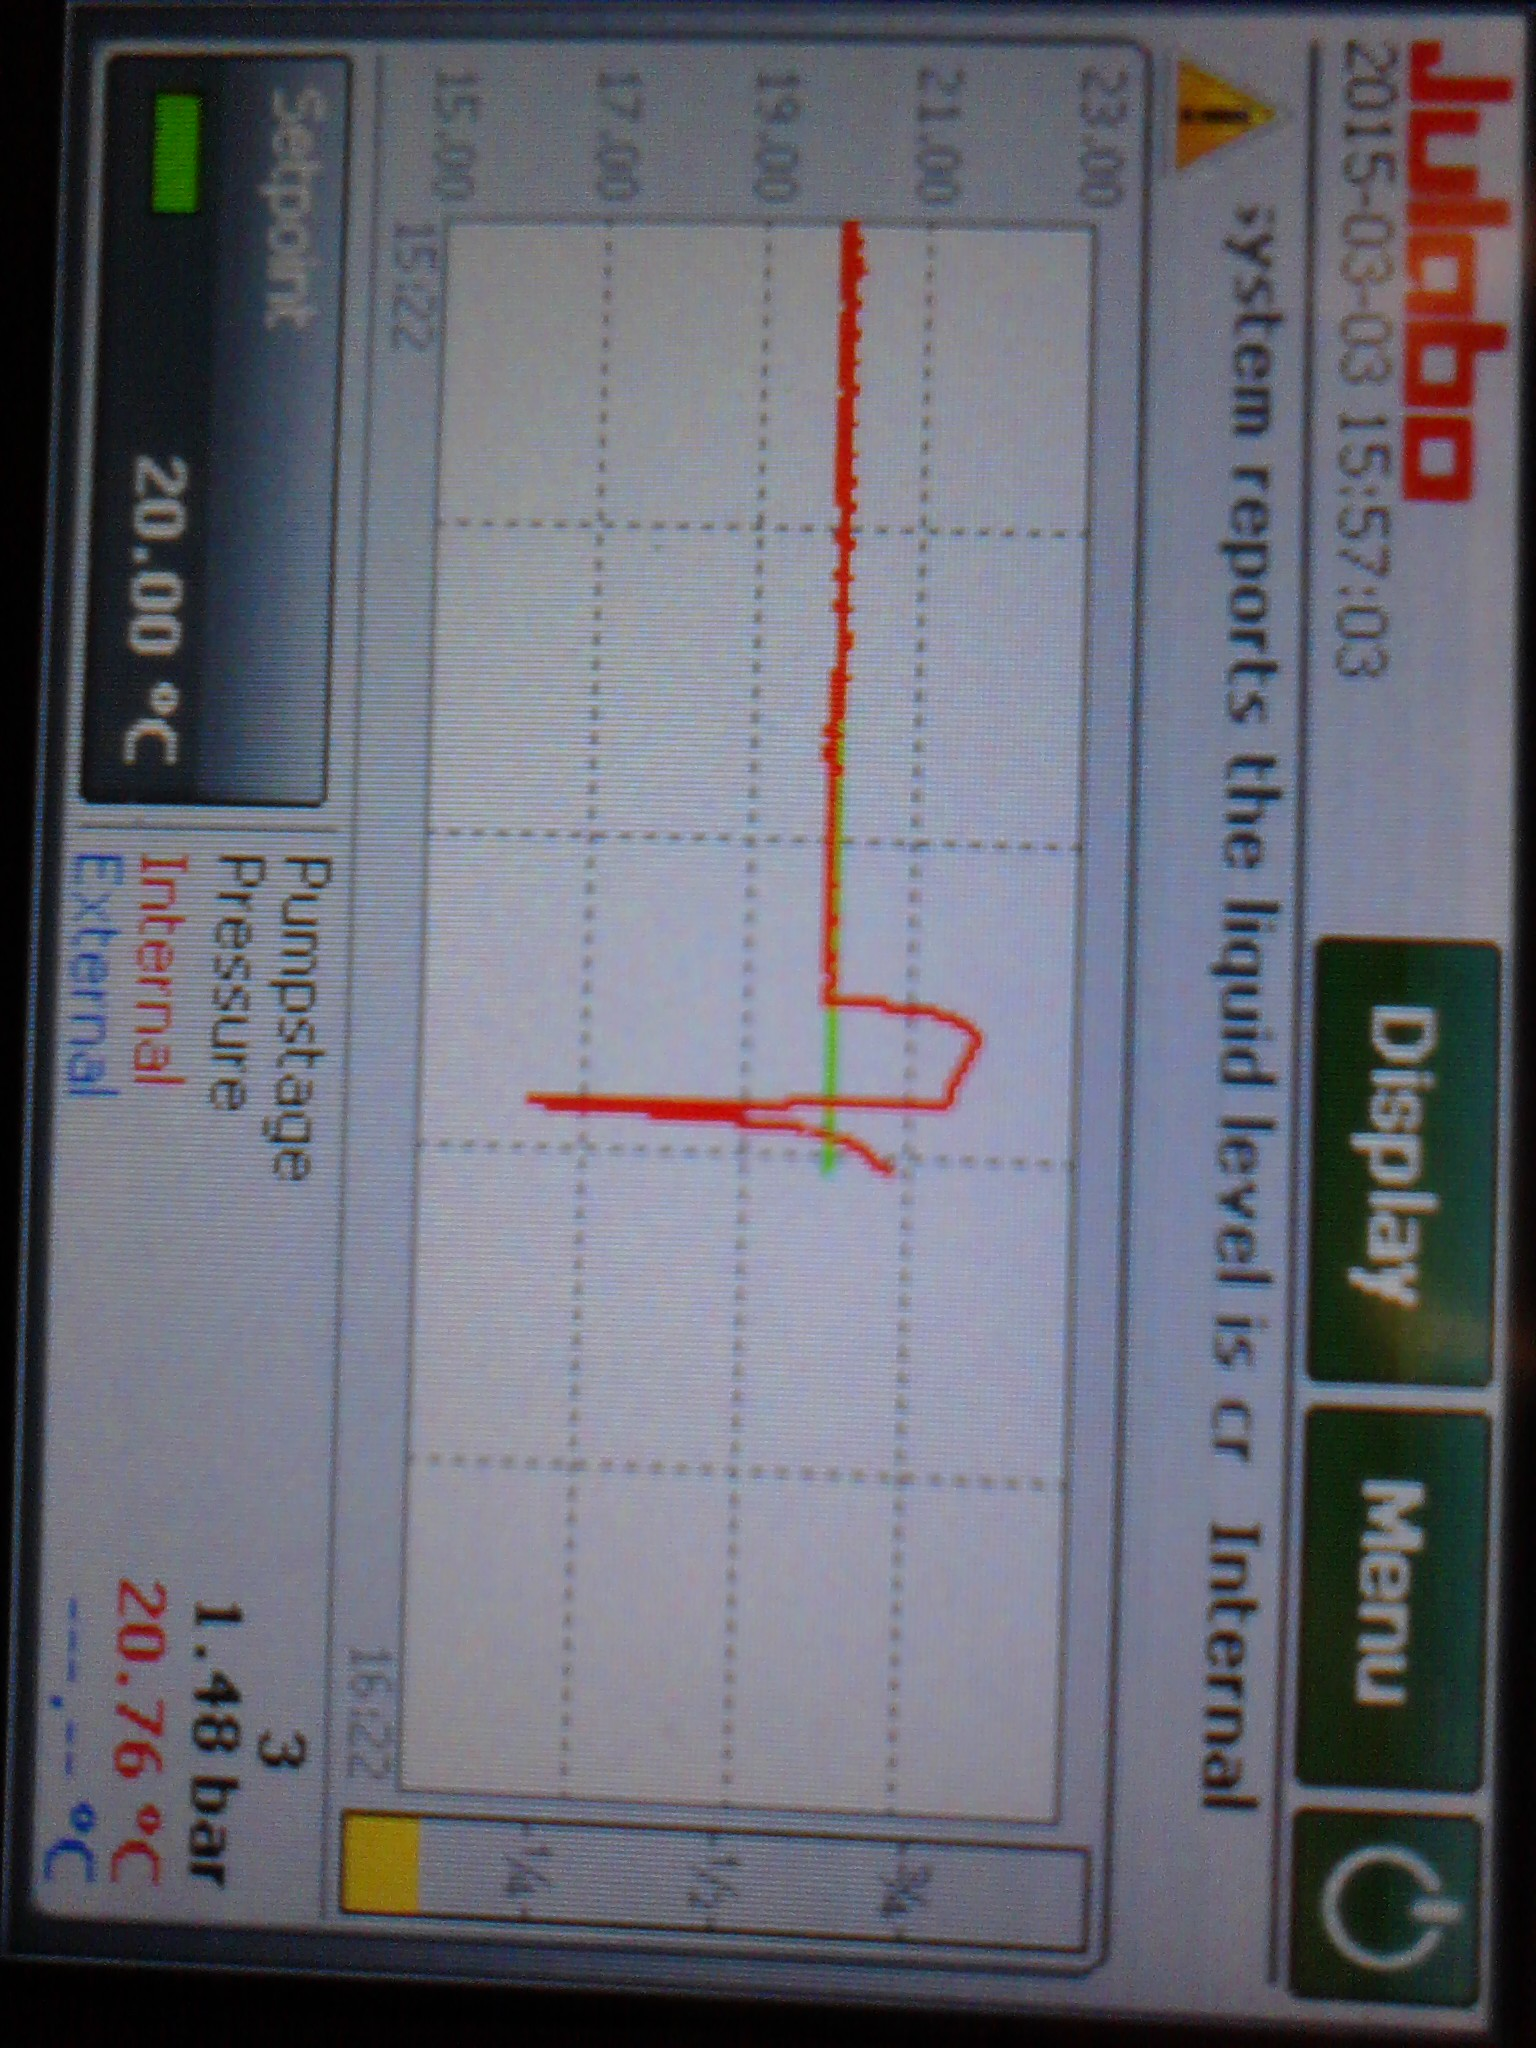
\includegraphics[angle=90,width=6cm]{figures/chiller_level1}
    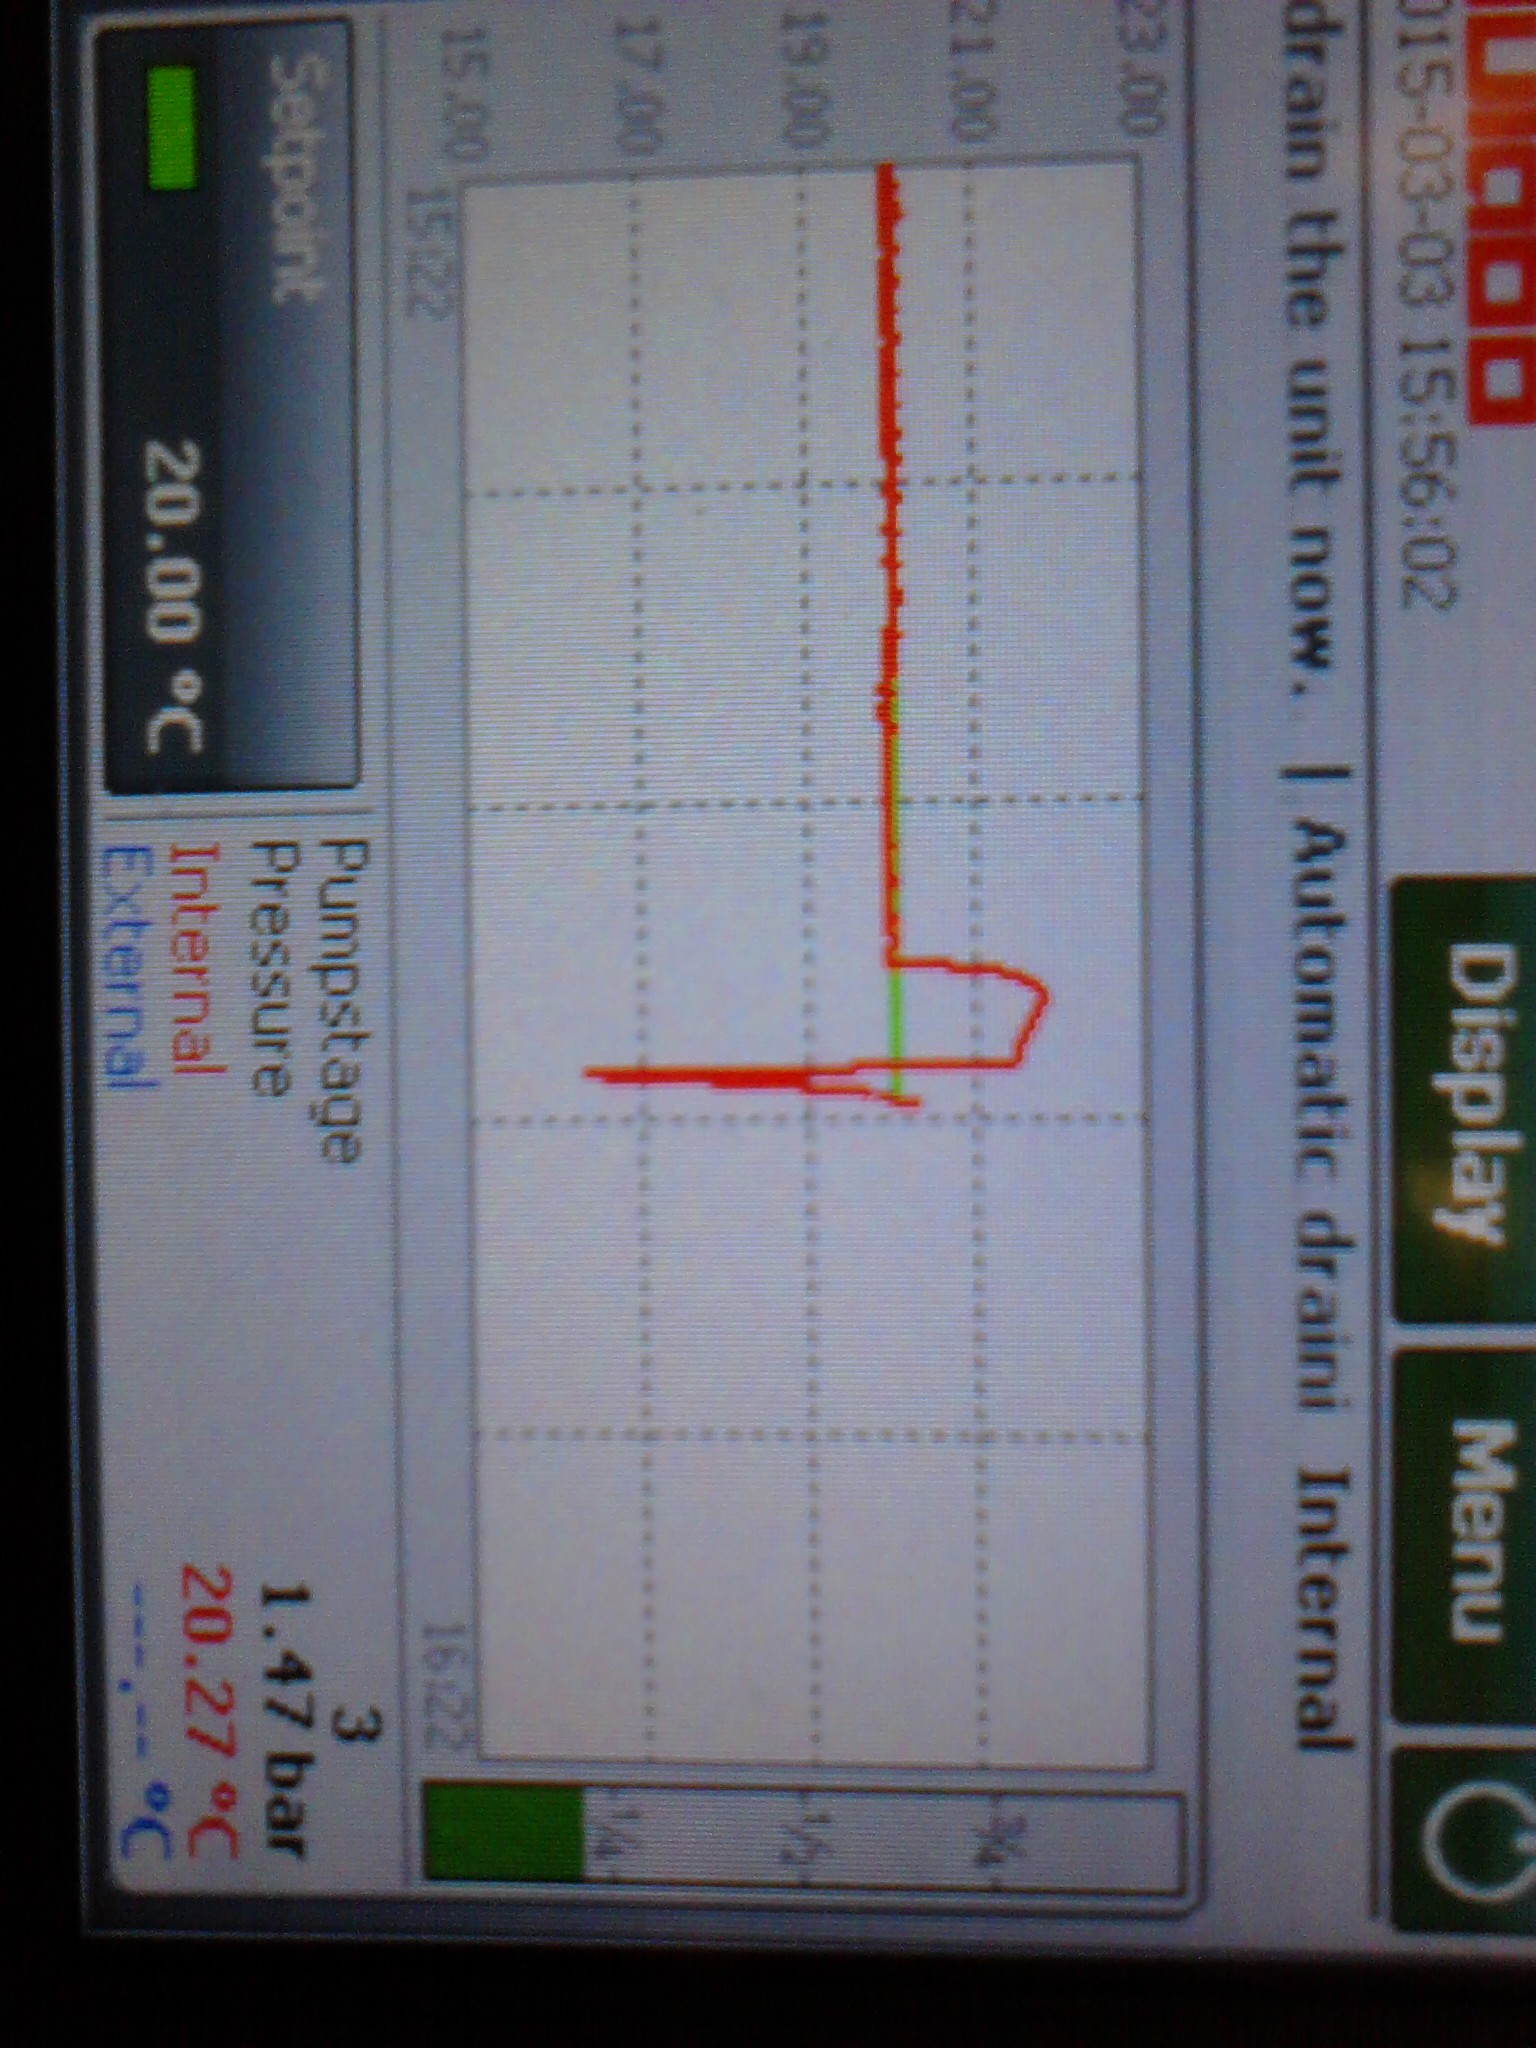
\includegraphics[angle=90,width=6cm]{figures/chiller_level2}
    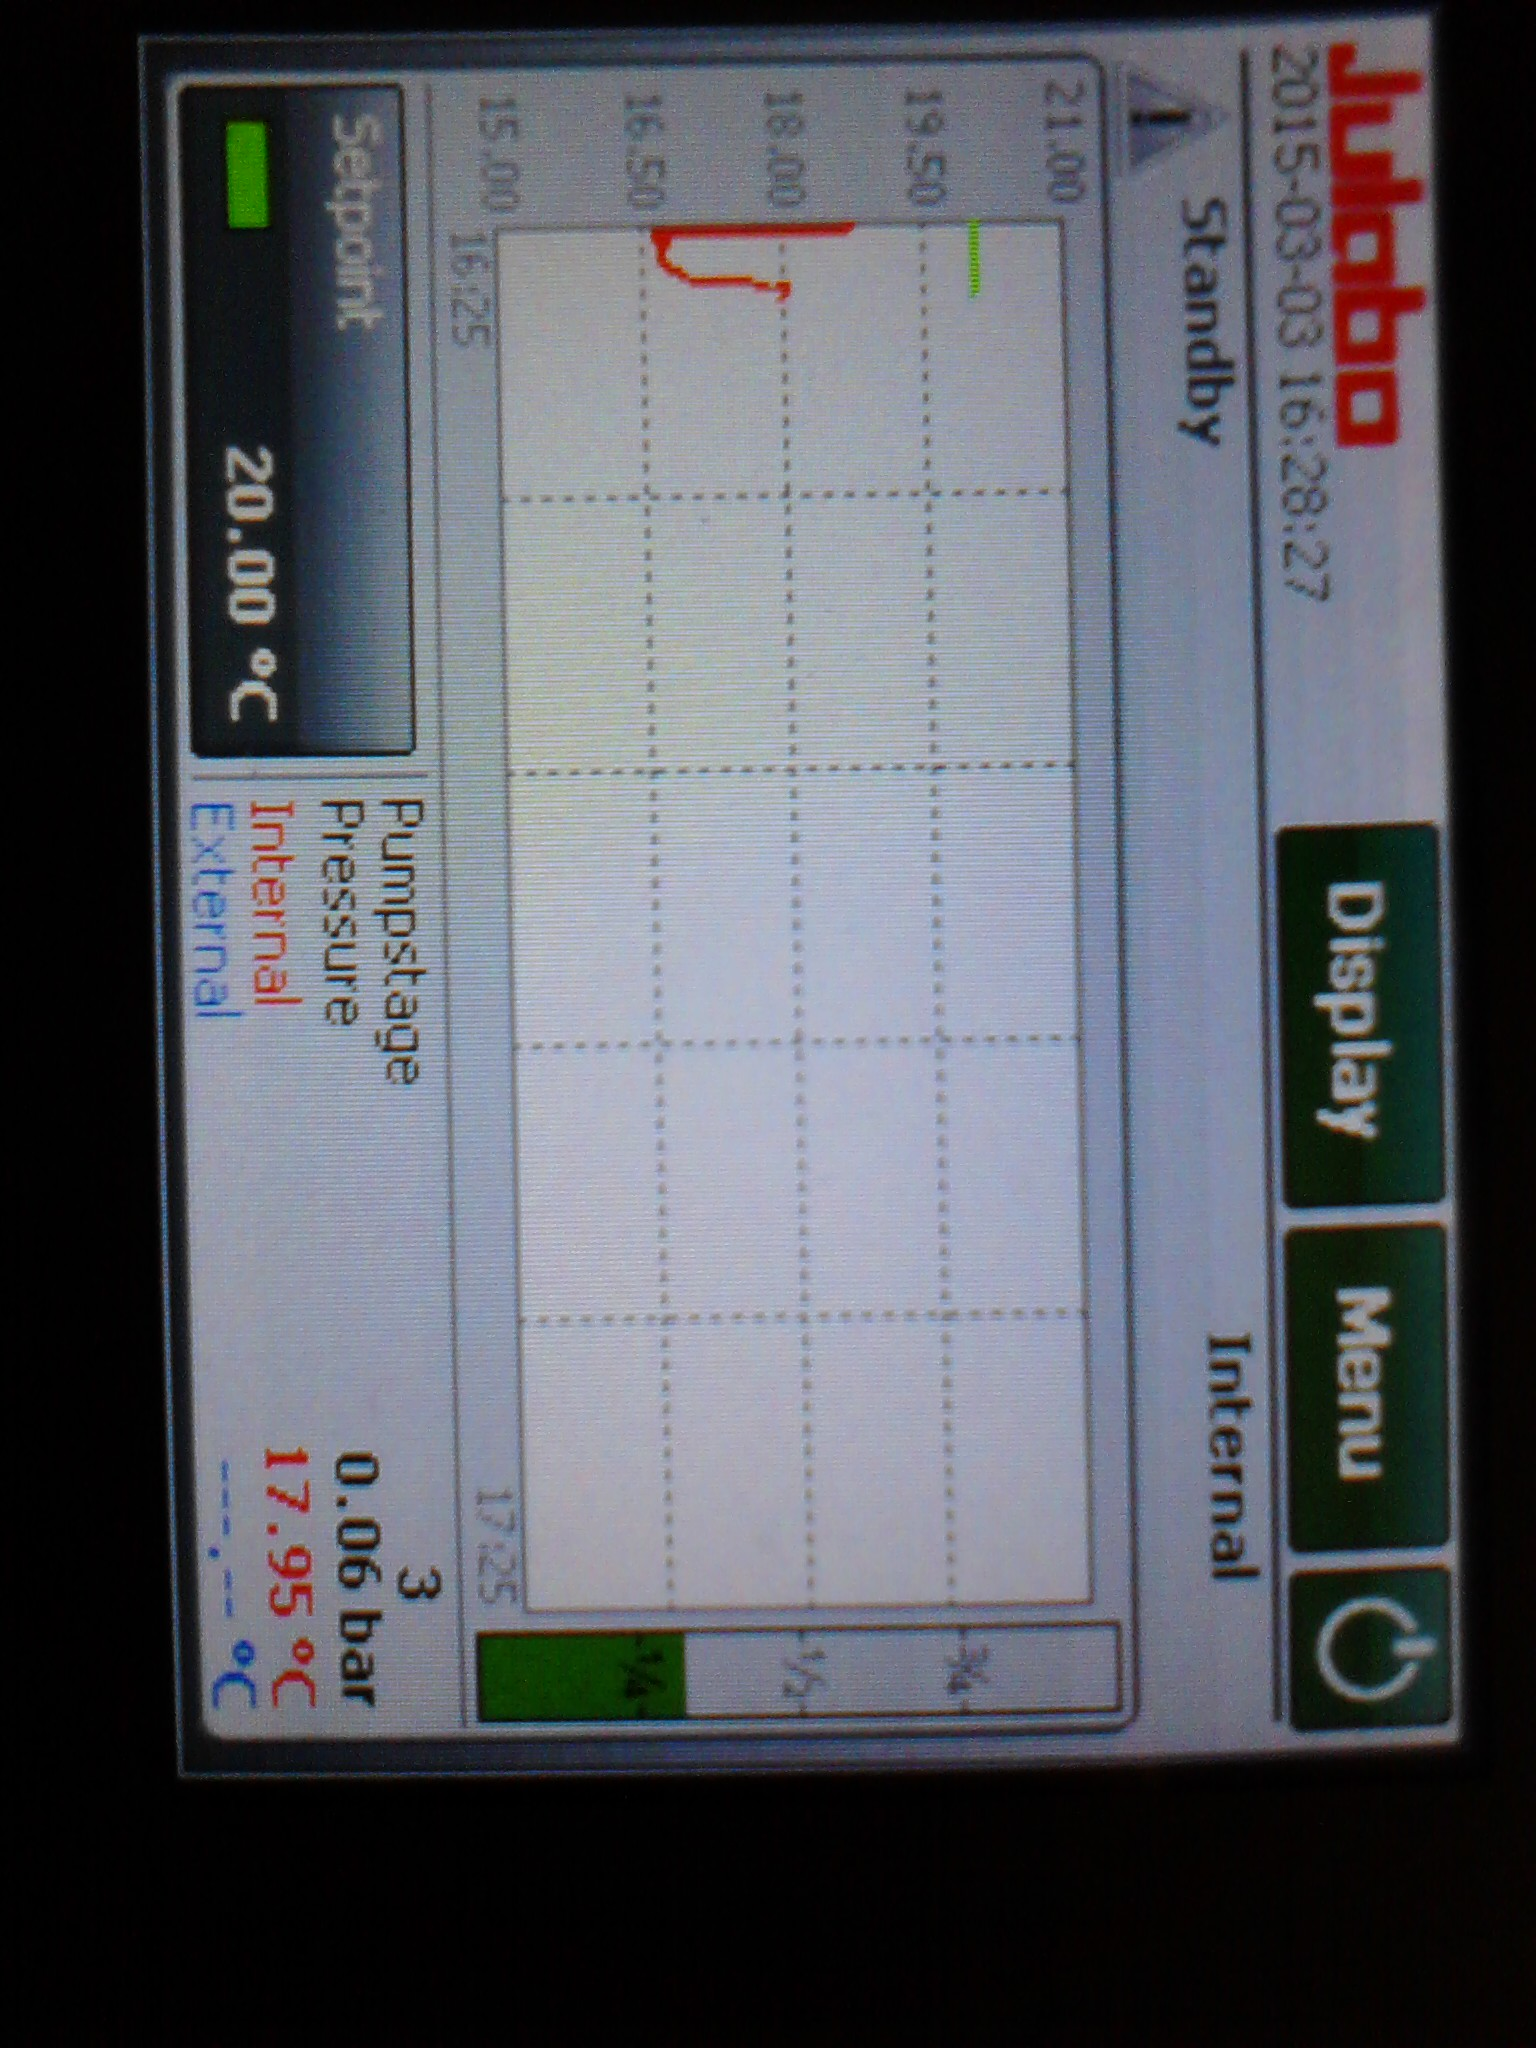
\includegraphics[angle=90,width=6cm]{figures/chiller_level3}
    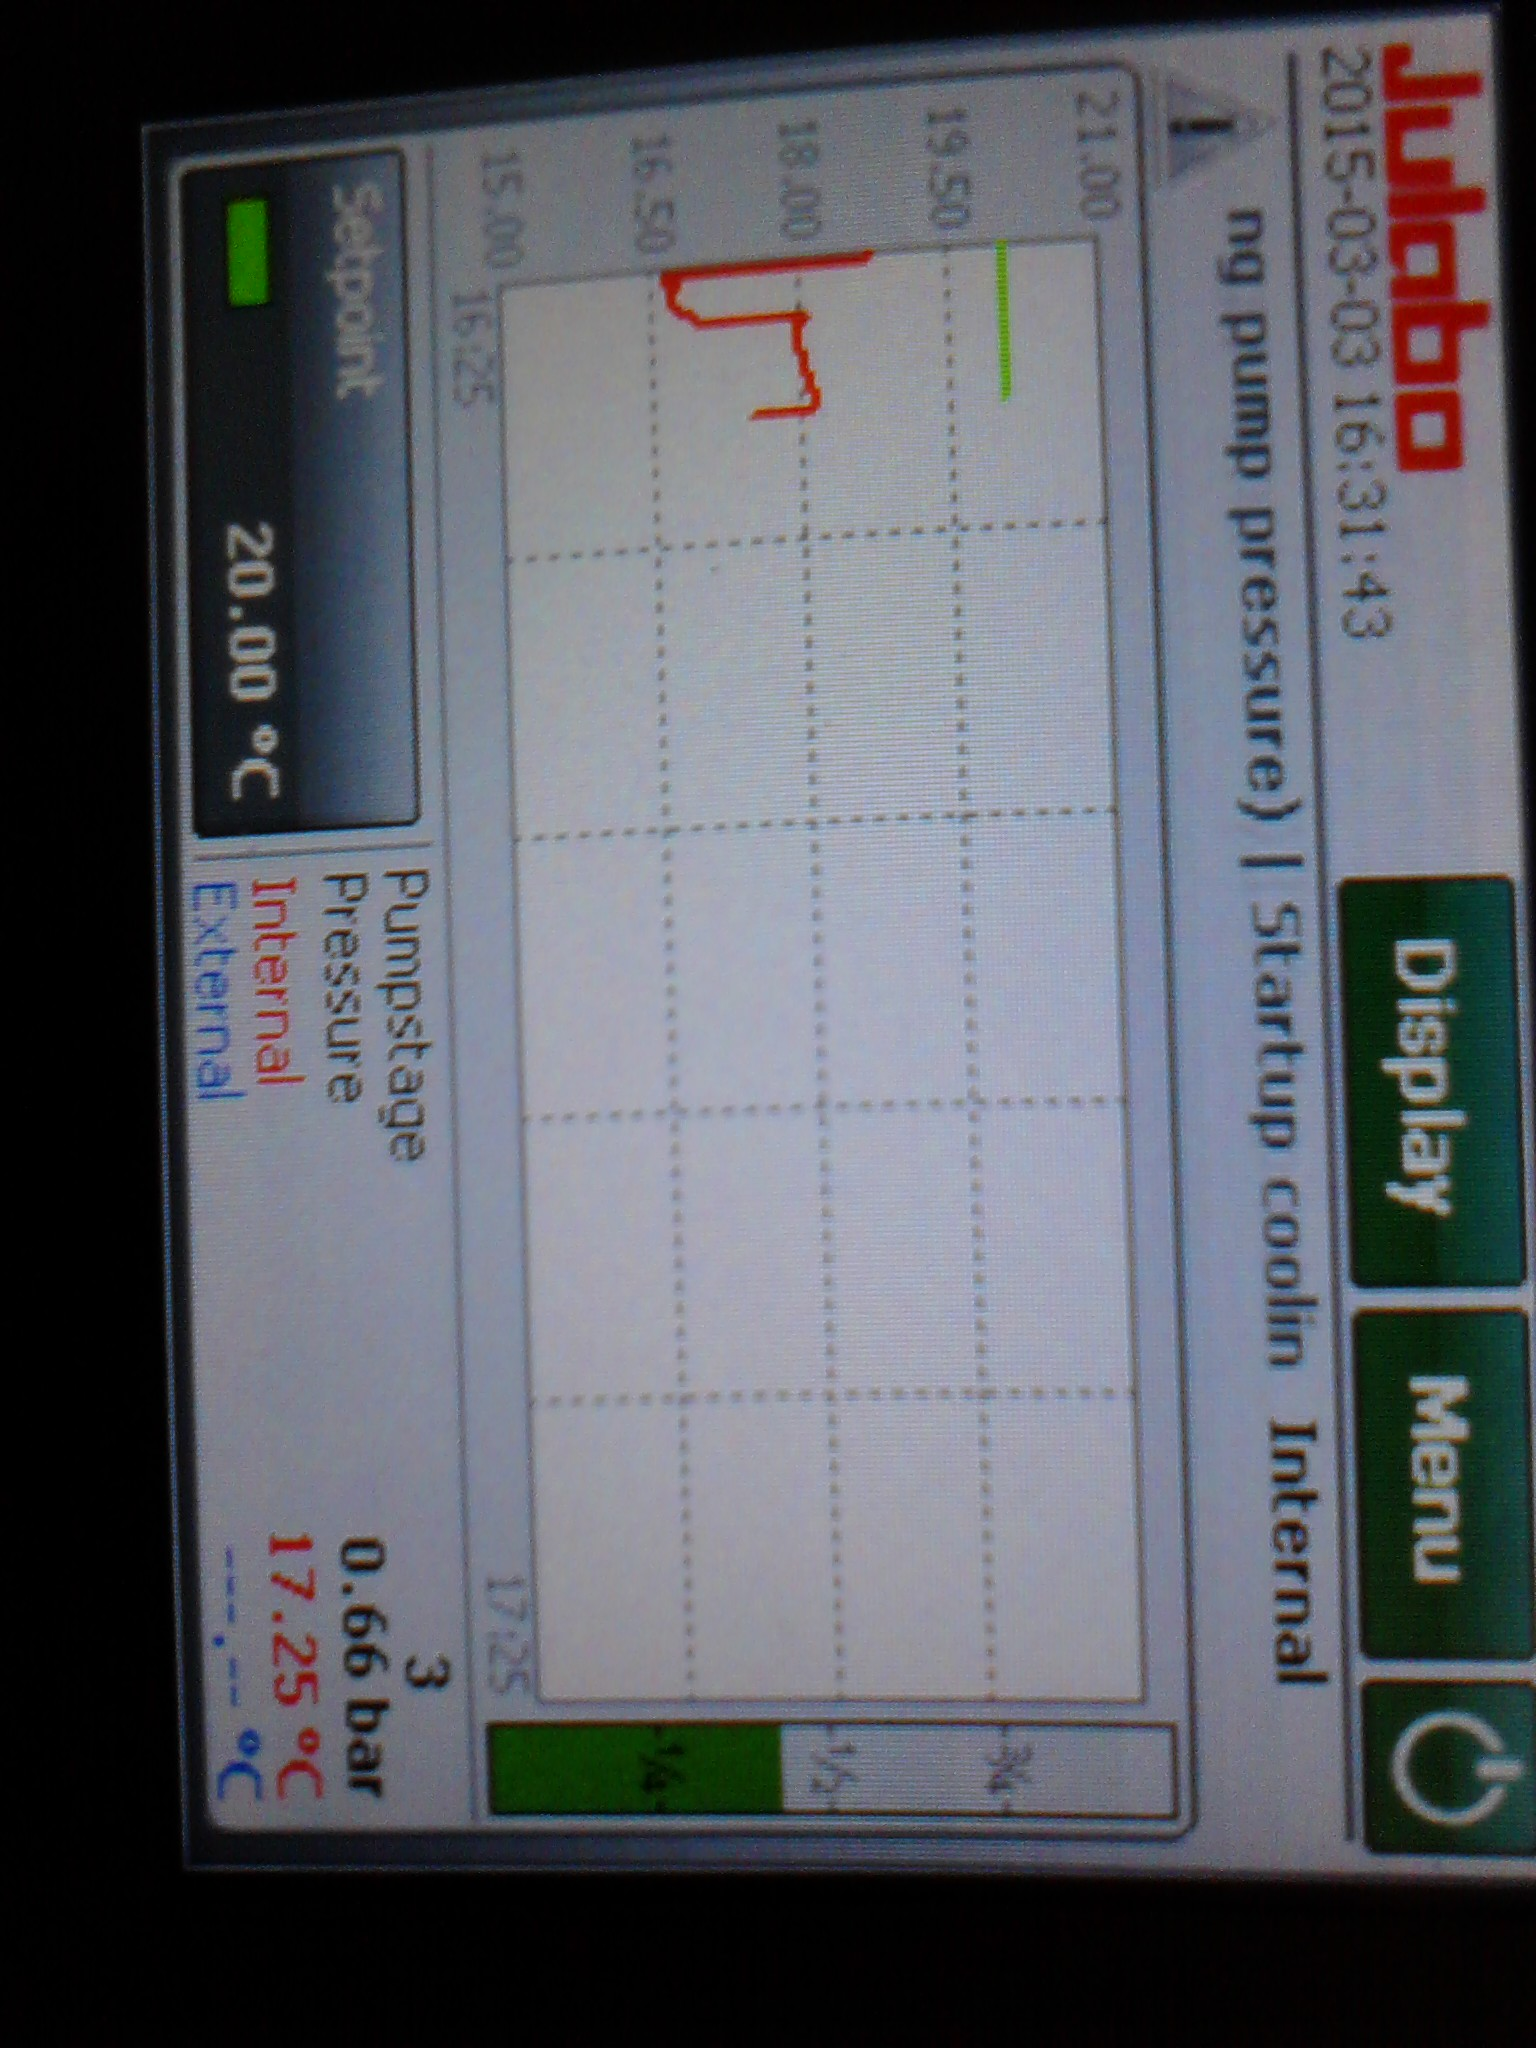
\includegraphics[angle=90,width=6cm]{figures/chiller_level4}
    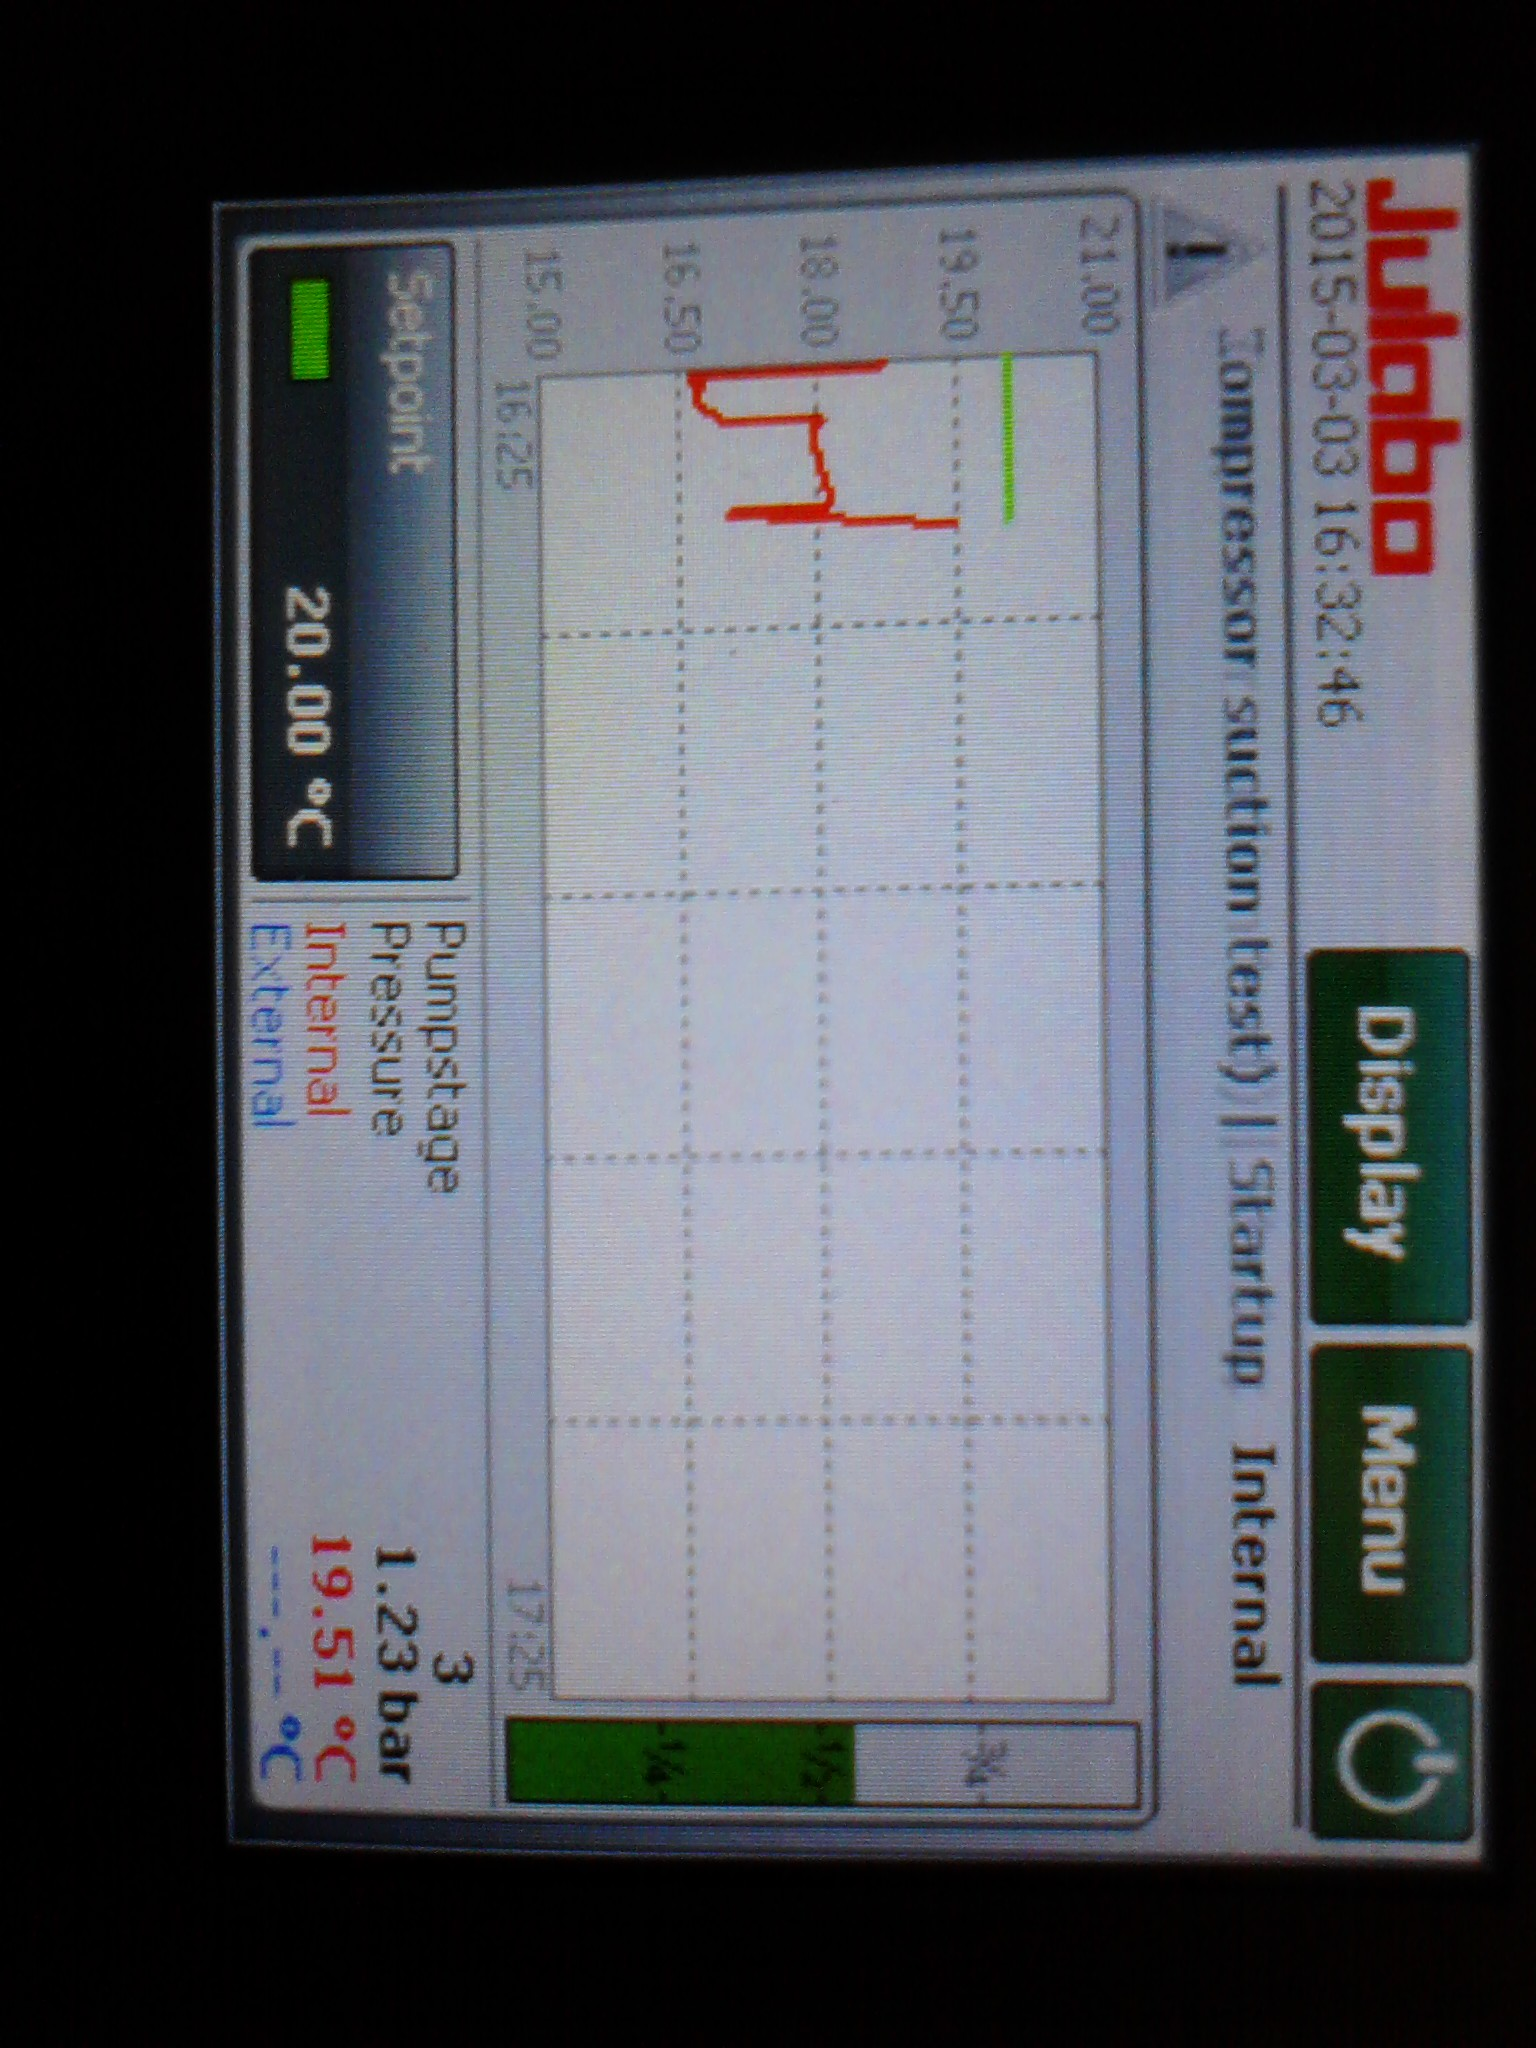
\includegraphics[angle=90,width=6cm]{figures/chiller_level5}
    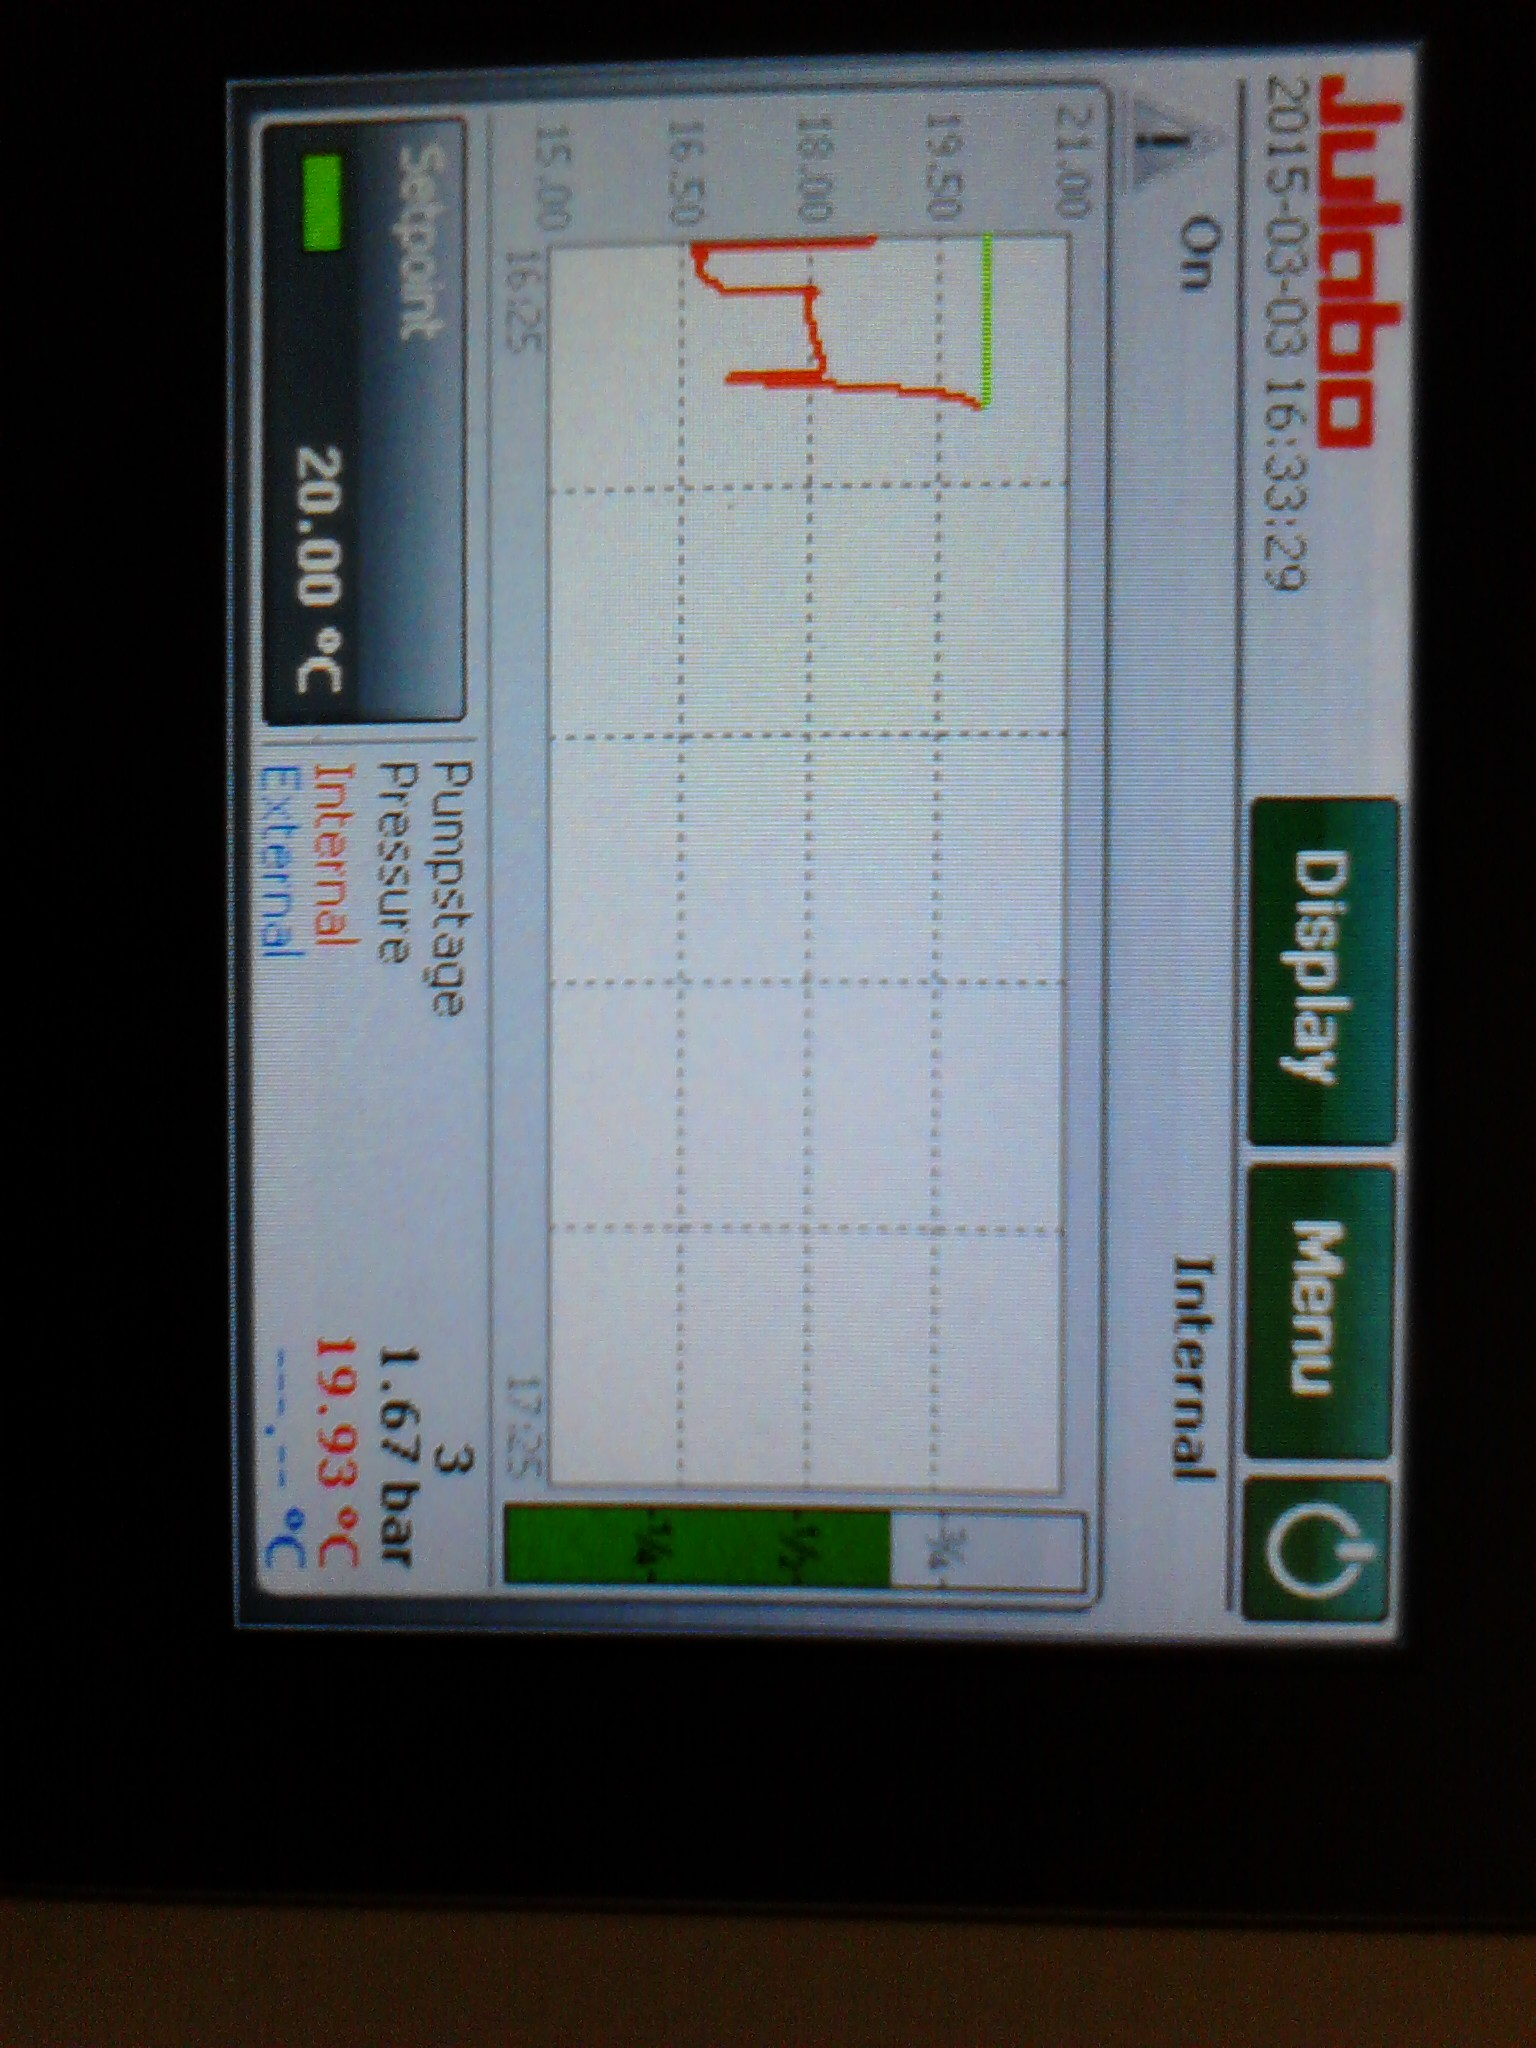
\includegraphics[angle=90,width=6cm]{figures/chiller_level6}
    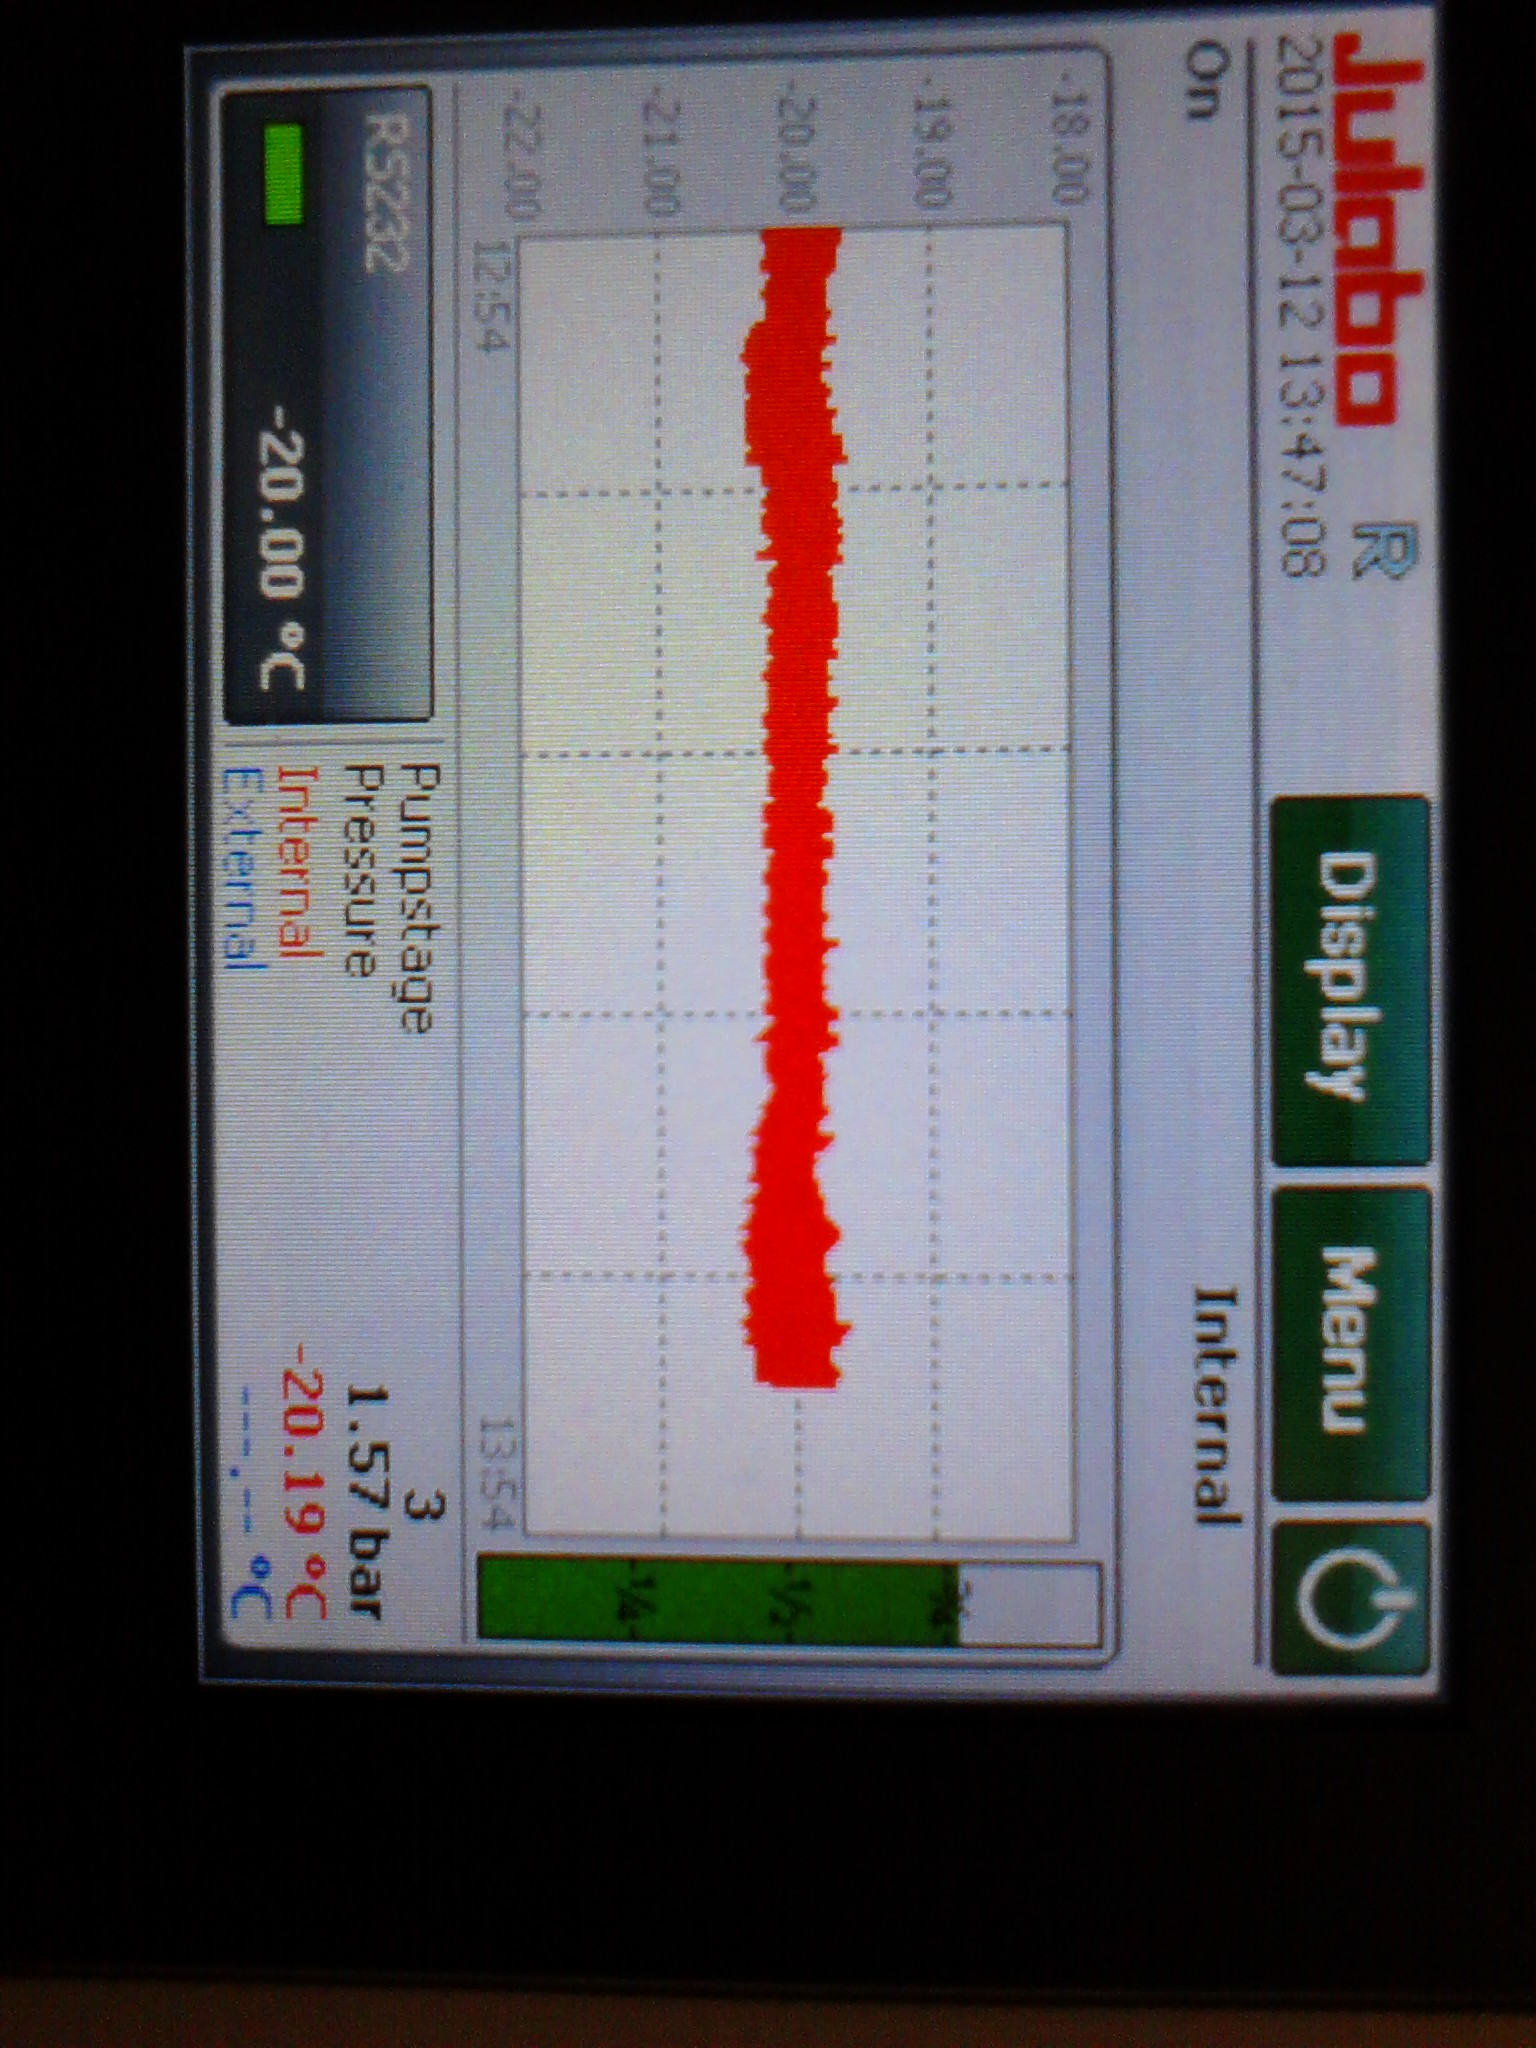
\includegraphics[angle=90,width=6cm]{figures/chiller_level7}
    \caption{Steps of the SVT chiller level indicator (green/yellow bar on right - it may be necessary to push the green ``Display'' button at the top to get to this view). Level 1 (first image) is the lowest level at which the chiller will continue to run, with a low level warning alarm. Levels 2--7 are levels for normal operation. Level 8 (not shown) will cause a high level warning alarm, but the chiller will continue to run. \label{fig:svt_chiller_level}}
\end{figure}

\subsection{Response to unexpected chiller trip}
\label{sec:proc_cooling_chillertrip}

\begin{enumerate}
    \item Look at the EPICS screens for the PLC. Check the alarm status fields for any PLC alarms. Also look at the software interlock screen and check the interlock status fields for any interlock faults. Call the SVT expert with the list of alarms.
    \item If the expert tells you to restart the chiller: Disable all PLC alarms that have tripped. Bypass and reset all software interlocks that have tripped. Start the chiller from its EPICS screen. As alarms clear, re-enable all alarms and interlocks that you disabled. If any alarm does not clear, call the SVT expert.
\end{enumerate}



\section{Motion}

\subsection{SVT Mover Operations}

Figure \ref{mover} shows the SVT Mover GUI.

\begin{itemize}
\item
Hit ``HOME'' button for Homing and confirm ``Homing Done'' in Status. It may take up to 3 minutes.
\item
Type in the destination of the layer 1 edge in mm in ``MOVE LAYER-1 TO'', and hit ``MOVE'' button.
\item
Type in a relative move value in mm in ``JOG LAYER-1 BY'', and hit either up or down triangle.
\item
Hit ``STOP'' to abort.
\end{itemize}

The positions of the stage, wire and Layer 1 sensor edge will be shown in ``SVT Position:'' in their respective coordinate.  Moving the SVT away from the home position is interlocked by beam conditions, shown by the interlock status light in the GUI.  Lack of safe interlock status will prevent motion of the SVT from the home position and loss of interlock will cause the SVT to return to home automatically.

\subsection{SVT Wire Scanner Operations}

When the beam is first delivered to Hall B, the vertical position of the beam is known to about 1 mm. Since we want to place the SVT layer 1 physical edge at 0.5 mm from the beam, SVT Wire Scanner is used to measure the beam position relative to the sensor edge with a precision of about 50~$\mu$m. The wire scanner has a 20 $\mu$m diameter gold-plated tungsten horizontal wire and a 30 $\mu$m diameter gold-plated tungsten angled wire. The angled wire is at 8.904 degrees to the horizontal wire, and is separeted by y=1.98 mm at the nominal beam position. The Y position of the beam can be measured directly from the horizontal wire. If $\Delta$Y is the apparent Y position difference of the measured beam ``gaussian'' centers, the X position of the beam can be obtained from X = ($\Delta$Y - 1.98)/tan(8.904).      

Wire scan should be repeated using the top wire and the bottom wire to check consistency. Once the beam offset values ($\Delta$X, $\Delta$Y) from the nominal beam position are measured, request MCC to move the beam using corrector magnets (MBC2H04V/H and MBC2H08V/H). Wire scan should be repeated to confirm the beam position.  As with any motion of the SVT, the ability to perform a wire scan may be interlocked by beam conditions, as shown by the interlock status light in the GUI.

\vskip 0.2 in

\noindent
\textbf{Setup}

\begin{itemize}
\item
MCC is not moving the beam or changing beam conditions.
\item
Ask MCC to mask BOM and Downstream Halo Counter in FSD.
\item
SVT power is turned off.
\item
ECal is operational.
\item
Downstream Halo Counter is operational.
\end{itemize}

\noindent
\textbf{Scan}

A wire scan can be performed from the SVT Wire Scan GUI (Figure \ref{scannergui}).

\begin{itemize}
\item 
Choose either TOP Wire or BOTTOM Wire.
\item
Choose either ECal or Halo Counter as the detector.
\item
Click ``START'' using the default values for Scan Range.
\item
When the status shows ``Done'', click ``Analyze'' button.
\end{itemize}

\begin{figure}[ht!]
\centering
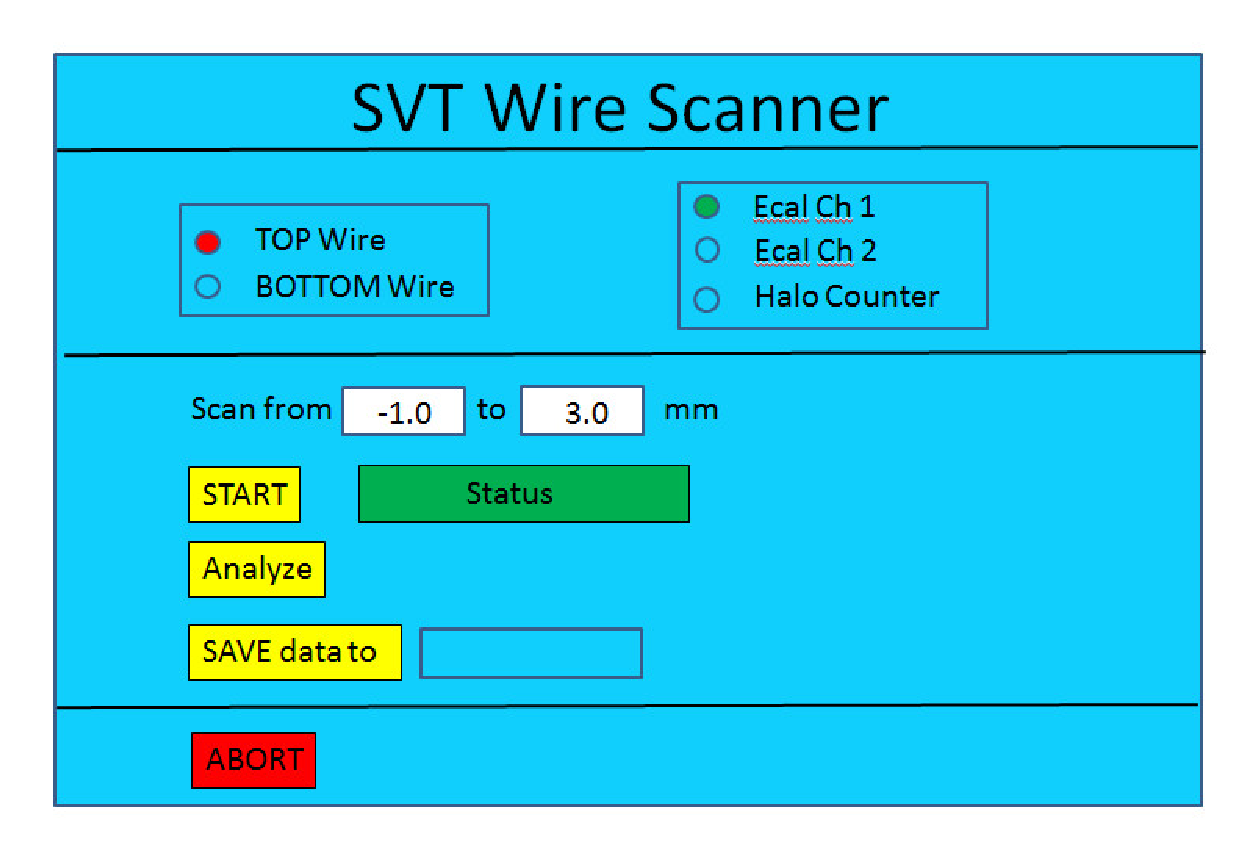
\includegraphics[width=10cm]{WireScannerGUI.eps}
\caption{SVT Wire Scanner GUI}
\label{scannergui}
\end{figure}

\end{document}
